\RequirePackage{silence}
\WarningFilter{remreset}{The remreset package}
%
% Eigentlicher Beginn des Dokuments
%
\documentclass[a4paper,
% pagebackref, % auskommentieren, falls Sie BibLaTeX benutzen
oneside, % Kommentarmarker entfernen, falls Sie einseitig binden wollen
% Der folgenden Zeile Kommentarmarker entfernen, falls Sie ein PDF-A benötigen
% pdfa,pdfapart=2,pdfaconformance=A,extension=pdf
]{book}
\usepackage[utf8]{inputenc}
\usepackage{lmodern}
\usepackage[T1]{fontenc}
\usepackage{ifthen}
%
% Alle Anpassungen der Titelseite erledigen Sie in der folgenden Datei
%

% 1. Personendaten
%
\newcommand{\myTitle}{Entwurf einer Power on Reset Schaltung mittels 130-nm-CMOS-Technologie}
%\newcommand{\mySubtitle}{Vorlage für die Bachelor-Arbeit}
%\newcommand{\myDegree}{Bachelor of Engineering}
%\newcommand{\myDegreeShort}{B.Eng.}
\newcommand{\myName}{Leon Hübner}
\newcommand{\myCompany}{Renesas Electronics Germany GmbH}
\newcommand{\myCompanyAddress}{Grenzstraße 28, 01109 Dresden}
\newcommand{\myId}{3005095}
\newcommand{\myExpert}{Dr. Stefan Getzlaff}
%\newcommand{\myProf}{Prof. Dr.-Ing. Arin Schlaumeier}
\newcommand{\myAcademy}{Staatliche Studienakademie Dresden}
% Vorsicht mit den Begriffen „Studiengang“ und „Studienrichtung“!
\newcommand{\myStudy}{Studienrgang Informationstechnik}
\newcommand{\myLocation}{Dresden} 
\newcommand{\myVersion}{Version 1.0}
% Abgabedatum
\newcommand{\mySubmissionDate}{\today}
% Datum der Selbständigkeitserklärung
% Abgabedatum und Datum der Selbständigkeitserklärung müssen nicht
% zwingend identisch sein. Sie können die Erklärung bereits ein paar
% Tage vorher (beispielsweise direkt nach dem Drucken und Binden)
% unterschreiben, während Sie die Arbeit erst später einreichen.
\newcommand{\myDeclarationDate}{28. Februar 2025}

%
% 2. Konfiguration
%
% 2a) Hat diese Arbeit einen Sperrvermerk?
%
\newboolean{lockflag}
\setboolean{lockflag}{false} % „false“, falls kein Sperrvermerk
%
% 2b) Soll statt des Abstracts ein Autorenreferat erscheinen?
%
\newboolean{extendedabstract}
\setboolean{extendedabstract}{false} % „true“, falls Autorenreferat
%
% 2c) Soll die Selbständigkeitserklärung vor das Inhaltsverzeichnis?
%     (Manche Gutachter wollen, dass die Selbständigkeitserklärung
%      am Anfang des Dokuments (direkt nach dem Titelblatt) steht.)
%
\newboolean{frontdeclaration}
\setboolean{frontdeclaration}{false} % „true“, für vorne

%
% 3. gescanntes Auftragsblatt einfügen
%
\newboolean{auftragsblatt}
\setboolean{auftragsblatt}{false}
% "false", falls kein Auftragsblatt eingebaut werden soll.
% Das Auftragsblatt muss sowohl im Printexemplar als auch in der
% elektronischen Version eingebunden werden! - In dieser Vorlage
% ist dafür der Platz zwischen der Zusammenfassung und dem
% Inhaltsverzeichnis vorgesehen.
% Für die elektronische Version bietet sich das Einbinden eines
% Scans an (true).
% Für die Printexemplare sollten Sie die Seitenzähler einfach nur
% um 2 erhöhen (true) und dann später die entsprechenden Blätter
% einlegen:
% * das Pflichtexemplar für das Archiv erhält das Original
% * die anderen Exemplare eine Kopie

%
% 4. Lorem Ipsum (am Ende auskommentieren!)
%
\usepackage{lipsum}

%
% 5. zu verwendende Pakete
%
% Hinweise zur Geometrie im Dokument beachten!
\usepackage{geometry}
\geometry{
	inner=40mm,
	outer=30mm,
	top=30mm
}
% Setzen Sie im folgenden die Option „htt“, wenn Sie wollen, dass
% Text in den Umgebungen \texttt und \ttfamily auch den Trennregeln
% des hyphenat-Pakets unterliegen sollen.
%\usepackage[htt]{hyphenat}
\usepackage{hyphenat}
\usepackage[ngerman,english]{babel}
\usepackage[babel]{csquotes}
% \usepackage{cite}
\usepackage{amsmath,amssymb,amstext,amsthm}
\usepackage{upgreek,units}
\usepackage{listings}
\lstset{ %
	basicstyle=\small,		% Schriftgröße im Kodeblock
	numberstyle=\tiny,
	numbers=left,			% Position der Zeilennummern
	stepnumber=1,			% Schrittweite der Zeilennummern („1“ bedeutet jede Zeile wird beschriftet)
	frame=tbl,				% Rahmen um Kodeblock (Standard: „single“)
	xleftmargin=15pt,
	numbersep=10pt,
	tabsize=4,				% Tabulatorgröße (4 Leerzeichen)
	captionpos=t,			% Position der Beschriftung
	breaklines=true,		% automatischer Zeilenumbruch
	breakatwhitespace=true,	% automatischer Zeilenumbruch nur an Leerzeichen, Tabulatoren, etc.
}
\renewcommand{\lstlistingname}{Quellkode}
\lstdefinestyle{plain}{frame=single, breaklines=true}
\lstdefinestyle{Java}{language=Java, basicstyle=\small, numbers=left, numberstyle=\tiny, numberblanklines=false, tabsize=4, xleftmargin=1.6em, frame=single, breaklines=true}
\usepackage{graphicx}
\usepackage{caption,subcaption}

\usepackage[hang,multiple]{footmisc}
\renewcommand{\footnotemargin}{1.2em}
\usepackage{longtable,booktabs,multirow,colortbl}
\usepackage{threeparttable} % Paket für Fußnoten in Tabellen
\usepackage{makecell}
\usepackage{rotating}
\usepackage{remreset}
\usepackage{savefnmark}
\usepackage{enumerate}
\usepackage[shortlabels]{enumitem}
\setlist{noitemsep, itemsep=3pt, topsep=0pt, partopsep=6pt}
\setenumerate{noitemsep, itemsep=3pt, topsep=0pt, partopsep=6pt}

\usepackage{thmtools}
\usepackage[nothm]{thmbox}
\usepackage[mathscr]{eucal}
\newtheoremstyle{style}
	{0}									%	Platz drüber
	{0}									%	Platz drunter
	{\normalfont}						%	Schriftstil
	{}									%	Einrückung
	{\normalfont\bfseries}				%	Theorembezeichner-Stil
	{:\\\vphantom{-}\vspace*{-.75em}\\}	%	Trennzeichen Bezeichner --> Inhalt
	{5pt plus 1pt minus 1pt}			%	Trennzeichen Text --> Theorem
	{{\normalfont\bfseries \thmname{#1}\thmnumber{ #2}\thmnote{ (#3)}}}
\theoremstyle{style}

\definecolor{HKS41-100}{cmyk}{1.0, 0.7, 0.1, 0.5}
% \definecolor{HKS41-90}{cmyk}{0.9, 0.63, 0.09, 0.45}
% \definecolor{HKS41-80}{cmyk}{0.8, 0.56, 0.08, 0.4}
% \definecolor{HKS41-70}{cmyk}{0.7, 0.49, 0.07, 0.35}
% \definecolor{HKS41-60}{cmyk}{0.6, 0.42, 0.06, 0.3}
% \definecolor{HKS41-50}{cmyk}{0.5, 0.35, 0.05, 0.25}
% \definecolor{HKS41-40}{cmyk}{0.4, 0.28, 0.04, 0.2}
% \definecolor{HKS41-30}{cmyk}{0.3, 0.21, 0.03, 0.15}
% \definecolor{HKS41-20}{cmyk}{0.2, 0.14, 0.02, 0.1}
% \definecolor{HKS41-10}{cmyk}{0.1, 0.07, 0.01, 0.05}
\definecolor{HKS44-100}{cmyk}{1.0, 0.5, 0.0, 0.0}
% \definecolor{HKS44-90}{cmyk}{0.9, 0.45, 0.0, 0.0}
% \definecolor{HKS44-80}{cmyk}{0.8, 0.4, 0.0, 0.0}
% \definecolor{HKS44-70}{cmyk}{0.7, 0.35, 0.0, 0.0}
% \definecolor{HKS44-60}{cmyk}{0.6, 0.3, 0.0, 0.0}
% \definecolor{HKS44-50}{cmyk}{0.5, 0.25, 0.0, 0.0}
% \definecolor{HKS44-40}{cmyk}{0.4, 0.2, 0.0, 0.0}
% \definecolor{HKS44-30}{cmyk}{0.3, 0.15, 0.0, 0.0}
% \definecolor{HKS44-20}{cmyk}{0.2, 0.1, 0.0, 0.0}
% \definecolor{HKS44-10}{cmyk}{0.1, 0.05, 0.0, 0.0}
% \definecolor{HKS36-100}{cmyk}{0.8, 0.9, 0.0, 0.0}
% \definecolor{HKS36-90}{cmyk}{0.72, 0.81, 0.0, 0.0}
% \definecolor{HKS36-80}{cmyk}{0.64, 0.72, 0.0, 0.0}
% \definecolor{HKS36-70}{cmyk}{0.56, 0.63, 0.0, 0.0}
% \definecolor{HKS36-60}{cmyk}{0.48, 0.54, 0.0, 0.0}
% \definecolor{HKS36-50}{cmyk}{0.4, 0.45, 0.0, 0.0}
% \definecolor{HKS36-40}{cmyk}{0.32, 0.36, 0.0, 0.0}
% \definecolor{HKS36-30}{cmyk}{0.24, 0.27, 0.0, 0.0}
% \definecolor{HKS36-20}{cmyk}{0.16, 0.18, 0.0, 0.0}
% \definecolor{HKS36-10}{cmyk}{0.08, 0.09, 0.0, 0.0}
% \definecolor{HKS33-100}{cmyk}{0.5, 1.0, 0.0, 0.0}
% \definecolor{HKS33-90}{cmyk}{0.45, 0.9, 0.0, 0.0}
% \definecolor{HKS33-80}{cmyk}{0.4, 0.8, 0.0, 0.0}
% \definecolor{HKS33-70}{cmyk}{0.35, 0.7, 0.0, 0.0}
% \definecolor{HKS33-60}{cmyk}{0.3, 0.6, 0.0, 0.0}
% \definecolor{HKS33-50}{cmyk}{0.25, 0.5, 0.0, 0.0}
% \definecolor{HKS33-40}{cmyk}{0.2, 0.4, 0.0, 0.0}
% \definecolor{HKS33-30}{cmyk}{0.15, 0.3, 0.0, 0.0}
% \definecolor{HKS33-20}{cmyk}{0.1, 0.2, 0.0, 0.0}
% \definecolor{HKS33-10}{cmyk}{0.05, 0.1, 0.0, 0.0}
\definecolor{HKS57-100}{cmyk}{1.0, 0.0, 0.9, 0.2}
% \definecolor{HKS57-90}{cmyk}{0.9, 0.0, 0.81, 0.18}
% \definecolor{HKS57-80}{cmyk}{0.8, 0.0, 0.72, 0.16}
% \definecolor{HKS57-70}{cmyk}{0.7, 0.0, 0.63, 0.14}
% \definecolor{HKS57-60}{cmyk}{0.6, 0.0, 0.54, 0.12}
% \definecolor{HKS57-50}{cmyk}{0.5, 0.0, 0.45, 0.1}
% \definecolor{HKS57-40}{cmyk}{0.4, 0.0, 0.36, 0.08}
% \definecolor{HKS57-30}{cmyk}{0.3, 0.0, 0.27, 0.06}
% \definecolor{HKS57-20}{cmyk}{0.2, 0.0, 0.18, 0.04}
% \definecolor{HKS57-10}{cmyk}{0.1, 0.0, 0.09, 0.02}
% \definecolor{HKS65-100}{cmyk}{0.65, 0.0, 1.0, 0.0}
% \definecolor{HKS65-90}{cmyk}{0.585, 0.0, 0.9, 0.0}
% \definecolor{HKS65-80}{cmyk}{0.52, 0.0, 0.8, 0.0}
% \definecolor{HKS65-70}{cmyk}{0.455, 0.0, 0.7, 0.0}
% \definecolor{HKS65-60}{cmyk}{0.39, 0.0, 0.6, 0.0}
% \definecolor{HKS65-50}{cmyk}{0.325, 0.0, 0.5, 0.0}
% \definecolor{HKS65-40}{cmyk}{0.26, 0.0, 0.4, 0.0}
% \definecolor{HKS65-30}{cmyk}{0.195, 0.0, 0.3, 0.0}
% \definecolor{HKS65-20}{cmyk}{0.13, 0.0, 0.2, 0.0}
% \definecolor{HKS65-10}{cmyk}{0.065, 0.0, 0.1, 0.0}
% \definecolor{HKS07-100}{cmyk}{0.0, 0.6, 1.0, 0.0}
% \definecolor{HKS07-90}{cmyk}{0.0, 0.54, 0.9, 0.0}
% \definecolor{HKS07-80}{cmyk}{0.0, 0.48, 0.8, 0.0}
% \definecolor{HKS07-70}{cmyk}{0.0, 0.42, 0.7, 0.0}
% \definecolor{HKS07-60}{cmyk}{0.0, 0.36, 0.6, 0.0}
% \definecolor{HKS07-50}{cmyk}{0.0, 0.3, 0.5, 0.0}
% \definecolor{HKS07-40}{cmyk}{0.0, 0.24, 0.4, 0.0}
% \definecolor{HKS07-30}{cmyk}{0.0, 0.18, 0.3, 0.0}
% \definecolor{HKS07-20}{cmyk}{0.0, 0.12, 0.2, 0.0}
% \definecolor{HKS07-10}{cmyk}{0.0, 0.06, 0.1, 0.0}
% \definecolor{HKS14-100}{cmyk}{0.0, 1.0, 1.0, 0.0}
% % % Benannte Farben
% \definecolor{white}{gray}{1.00}
% \definecolor{black}{gray}{0.00}
% \definecolor{skyblue}{cmyk}{0.4, 0.2, 0.0, 0.0}             % HKS44-40
\definecolor{blue}{cmyk}{1.0, 0.5, 0.0, 0.0}                % HKS44-100
% \definecolor{lightblue}{cmyk}{0.7, 0.35, 0.0, 0.0}          % HKS44-70
% \definecolor{darkblue}{rgb}{0.04, 0.16, 0.32}               % 
% \definecolor{extradarkblue}{cmyk}{1.00, 0.70, 0.10, 0.50}   % HKS41-100
\definecolor{darkgreen}{cmyk}{1.0, 0.0, 0.9, 0.2}           % HKS57-100
% \definecolor{green}{cmyk}{0.65, 0.0, 1.0, 0.0}              % HKS65-100
% \definecolor{purple}{cmyk}{0.5, 1.0, 0.0, 0.0}              % HKS33-100
% \definecolor{indigo}{cmyk}{0.8, 0.9, 0.0, 0.0}              % HKS36-100
% \definecolor{gray}{gray}{0.59}
% \definecolor{darkgray}{gray}{0.50}
% \definecolor{darkcyan}{cmyk}{0.87, 0.4, 0.4, 0.0}
% \definecolor{cyan}{cmyk}{0.78, 0.19, 0.01, 0.0}
% \definecolor{lightcyan}{cmyk}{0.39, 0.095, 0.005, 0.0}
% \definecolor{extralightcyan}{cmyk}{0.16, 0.1, 0.0, 0.0}
\definecolor{lightred}{rgb}{1.0, 0.9, 0.9} % Helleres Rot
\definecolor{lightyellow}{rgb}{1.0, 1.0, 0.7} % Helleres Gelb
% 
% \definecolor{shadeThe}{cmyk}{.1,.05,0,0}		% HKS44_10%
% \definecolor{frameThe}{cmyk}{.7,.35,0,0}		% HKS44_70%
% \definecolor{shadeDef}{cmyk}{.07,0,.1,0}		% HKS65_10%
% \definecolor{frameDef}{cmyk}{.2,0,.4,0}			% HKS65_40%
% \definecolor{shadeThm}{cmyk}{.05,.1,0,0}		% HKS33_10%
% \definecolor{frameThm}{cmyk}{.2,.4,0,0}			% HKS33_40%
% \definecolor{shadeLem}{cmyk}{0,.06,.1,0}		% HKS07_10%
% \definecolor{frameLem}{cmyk}{0,.24,.4,0}		% HKS07_40%
% \definecolor{shadeCor}{cmyk}{.1,.07,.01,.05}	% HKS41_10%
% \definecolor{frameCor}{cmyk}{.4,.28,.04,.2}		% HKS41_40%
% \definecolor{shadePrf}{cmyk}{.08,.09,0,0}		% HKS36_10%
% \definecolor{framePrf}{cmyk}{.32,.36,0,0}		% HKS36_40%
% \definecolor{shadeAss}{cmyk}{.1,0,.09,.02}		% HKS57_10%
% \definecolor{frameAss}{cmyk}{.34,0,.36,.08}		% HKS57_40%

\declaretheorem[name=Arbeitsthese,shaded={rulecolor=frameThe,rulewidth=1pt,bgcolor=shadeThe,textwidth=\textwidth-2pt}]{myworkingthesis}
\declaretheorem[name=Annahme,numbered=no,shaded={rulecolor=frameAss,rulewidth=1pt,bgcolor=shadeAss,textwidth=\textwidth-2pt}]{myassertion}
\declaretheorem[numberwithin=section,name=Definition,shaded={rulecolor=frameDef,rulewidth=1pt,bgcolor=shadeDef,textwidth=\textwidth-2pt}]{mydef}
\declaretheorem[sibling=mydef,name=Theorem,shaded={rulecolor=frameThm,rulewidth=1pt,bgcolor=shadeThm,textwidth=\textwidth-2pt}]{mytheorem}
\declaretheorem[sibling=mydef,name=Lemma,shaded={rulecolor=frameLem,rulewidth=1pt,bgcolor=shadeLem,textwidth=\textwidth-2pt}]{mylemma}
\declaretheorem[sibling=mydef,name=Korollar,shaded={rulecolor=frameCor,rulewidth=1pt,bgcolor=shadeCor,textwidth=\textwidth-2pt}]{mycorollary}
\declaretheorem[sibling=mydef,name=Beweis,shaded={rulecolor=framePrf,rulewidth=1pt,bgcolor=shadePrf,textwidth=\textwidth-2pt}]{myproof}
\declaretheorem[sibling=mydef,name=Abbildung]{myfig}

\AtBeginDocument{\numberwithin{lstlisting}{section}}
\newcounter{thmhelper}[section]
\newcounter{thesiscount}
\makeatletter
	\@removefromreset{footnote}{chapter}
\makeatother

\usepackage{wrapfig}

\newcommand{\inlinecode}[1]{%
	\colorbox{extralightcyan}{%
		\texttt{#1}%
	}%
}%

\newcommand{\mytable}[0]{%
	\setcounter{table}{\thethmhelper}%
	\addtocounter{thmhelper}{1}%
}%
%\newcommand{\myequation}[0]{%
%	\setcounter{equation}{\thethmhelper}%
%	\addtocounter{thmhelper}{1}%
%}%
\newenvironment{workingthesis}[1][]{%
	\addtocounter{thesiscount}{1}%
	\begin{myworkingthesis}[#1]}{\end{myworkingthesis}%
}%
\newenvironment{assertion}[1][]{%
	\begin{myassertion}[#1]}{\end{myassertion}%
}%
\newenvironment{definition}[1][]{%
	\addtocounter{thmhelper}{1}%
	\begin{mydef}[#1]}{\end{mydef}%
}%
\newenvironment{theorem}[1][]{%
	\addtocounter{thmhelper}{1}%
	\begin{mytheorem}[#1]}{\end{mytheorem}%
}%
\newenvironment{lemma}[1][]{%
	\addtocounter{thmhelper}{1}%
	\begin{mylemma}[#1]}{\end{mylemma}%
}%
\newenvironment{corollary}[1][]{%
	\addtocounter{thmhelper}{1}%
	\begin{mycorollary}[#1]}{\end{mycorollary}%
}%
\renewenvironment{proof}[1][]{%
	\addtocounter{thmhelper}{1}%
	\begin{myproof}[#1]}{%
		\nopagebreak%
		\\%
		{} \qed%
	\end{myproof}%
}%
\newcommand{\comment}[1]{%
	\, {} \hfill {\, }%
	{\color{gray}\begin{thmbox}[S]{\textit{Kommentar}}%
		\setlength{\parindent}{-0.3em}%
		\textit{#1}%
	\end{thmbox}}%
	\vspace{1em}%
}%
\renewcommand{\example}[1]{%
	\, {} \hfill {\, }%
	\begin{thmbox}[S]{\textit{Beispiel}}%
		\setlength{\parindent}{-0.2em}%
		#1%
	\end{thmbox}%
	\vspace{1em}%
}%

\makeatletter%
	\def\Autoref#1{%
		\begingroup%
			\def\reserved@a{\cpttrimspaces{#1}}%
			\ifcsndefTF{r@#1}{%
				\xaftercsname{\expandafter\testreftype\@fourthoffive}%
				{r@\reserved@a}.\\{#1}%
			}{%
				\ref{#1}%
			}%
		\endgroup%
	}%
	\def\testreftype#1.#2\\#3{%
		\ifcsndefTF{#1autorefname}{%
			\def\reserved@a##1##2\@nil{%
				\uppercase{\def\ref@name{##1}}%
				\csn@edef{#1autorefname}{\ref@name##2}%
				\autoref{#3}%
			}%
			\reserved@a#1\@nil%
		}{%
			\autoref{#3}%
		}%
	}%
\makeatother%

\usepackage{imakeidx}
\makeindex

\usepackage{tocloft}
\usepackage{chngcntr}
%
\setlength{\cftfignumwidth}{1.2cm}  % Breite des Nummerierungsbereichs für Abbildungen
\setlength{\cfttabnumwidth}{1.2cm}  % Breite des Nummerierungsbereichs für Tabellen

% Für durchgehende Nummerrierung 
% \counterwithout{figure}{chapter}
% \counterwithout{table}{chapter}


\setlength{\cftfigindent}{0pt} % Einrückung der Abbildungsnummer entfernen (optional)
\setlength{\cftbeforefigskip}{0pt} % Abstand zwischen den Einträgen entfernen

% Für Nummerrierung nach Kapitel 
\numberwithin{figure}{section}
\numberwithin{table}{section}
\numberwithin{table}{section}
\numberwithin{equation}{section}
\addto\extrasngerman{%
	\renewcommand{\figureautorefname}{Abbildung}
	\renewcommand{\tableautorefname}{Tabelle}
	\renewcommand{\subsectionautorefname}{Unterabschnitt}%
	\renewcommand{\sectionautorefname}{Abschnitt}%
	\renewcommand{\chapterautorefname}{Kapitel}%
	\renewcommand{\partautorefname}{Teil}%
}
\pagecolor{white}
\usepackage{pdfpages}
\makeatletter
\renewcommand{\@chapter}[2][]{%
    \ifnum\c@secnumdepth>\m@ne
        \if@mainmatter
            \refstepcounter{chapter}%
            \typeout{\@chapapp\space\thechapter.}%
            \addcontentsline{toc}{chapter}{\protect\numberline{\thechapter}#2}%
        \else
            \addcontentsline{toc}{chapter}{#2}%
        \fi
    \else
        \addcontentsline{toc}{chapter}{#2}%
    \fi
    \chaptermark{#1}%
    \if@twocolumn
        \@topnewpage[\@makechapterhead{#2}]%
    \else
        \@makechapterhead{#2}%
        \@afterheading
    \fi
    \addtocontents{lof}{\protect\addvspace{0pt}} % Unterdrückt den Abstand im Abbildungsverzeichnis
}\makeatother
\newcommand{\imgbox}[7]{%
	\begin{wrapfigure}{#1}{#2}%
		\centering%
		\vspace{-0.5em}%
		\includegraphics[width=#3]{figures/#4}%
		\vspace{-1.0em}%
		\addtocounter{thmhelper}{1}%
		\setcounter{figure}{\thethmhelper}%
		\caption[#6]{#7}\label{fig:#5}%
		\vspace{-0.5em}%
	\end{wrapfigure}%
}%
\newcommand{\img}[5]{%
	\begin{figure}[htbp]%
		%% Eine normale Abbildung
		%%  #1 Breite der Abbildung
		%%  #2 Abbildung
		%%  #3 Label
		%%  #4 TOC-Beschriftung
		%%  #5 Beschriftung
		%%
		%% (Falls es komisch aussieht, setzen Sie
		%%  nur „t“ oder „tb“ statt „htbp“)
		\vspace{2.5em}%
		\centering%
		\includegraphics[width=#1]{figures/#2}
		\vspace{-0.5em}%
		\addtocounter{thmhelper}{1}%
		\setcounter{figure}{\thethmhelper}%
		\caption[#4]{#5}\label{fig:#3}%
		\vspace{1.5em}%
	\end{figure}%
}%
\newcommand\imgAB[9]{%
	%% LaTeX-Hexerei mit \imgABcontinued
	%% (wegen mehr als 9 Parametern)
	\def\tmpvalone{#1}%
	\def\tmpvaltwo{#2}%
	\def\tmpvalthr{#3}%
	\def\tmpvalfou{#4}%
	\def\tmpvalfiv{#5}%
	\def\tmpvalsix{#6}%
	\def\tmpvalsev{#7}%m
	\def\tmpvalnin{#9}%
	\imgABcontinued%
}%
\newcommand{\imgABcontinued}[2]{%
	\begin{figure}[htbp]%
		\vspace{2.5em}%
		\centering%
		\begin{subfigure}[t]{\tmpvalfou\textwidth}%
			\centering%
			\includegraphics[width=\tmpvalfiv]{figures/\tmpvalsix}%
			\caption{\tmpvalsev}\label{fig:\tmpvalone-A}%
		\end{subfigure}%
		\hfill~%
		\begin{subfigure}[t]{\tmpvaleig\textwidth}%
			\centering%
			\includegraphics[width=\tmpvalnin]{figures/#1}%
			\caption{#2}\label{fig:\tmpvalone-B}%
		\end{subfigure}%
		\vspace{-0.5em}%
		\addtocounter{thmhelper}{1}%
		\setcounter{figure}{\thethmhelper}%
		\caption[\tmpvaltwo]{\tmpvalthr}\label{fig:\tmpvalone}%
		\vspace{1.5em}%
	\end{figure}%
}%
\newcommand{\imgABstack}[9]{%
	\begin{figure}[htbp]%
		\vspace{2.5em}%
		\centering%
		\begin{subfigure}[t]{\textwidth}%
			\centering%
			\includegraphics[width=#4]{figures/#5}%
			\caption{#6}\label{fig:#1-A}%
		\end{subfigure}%
		\\%
		\vspace{2em}%
		\begin{subfigure}[t]{\textwidth}%
			\centering%
			\includegraphics[width=#7]{figures/#8}%
			\caption{#9}\label{fig:#1-B}%
		\end{subfigure}%
		\vspace{-0.5em}%
		\addtocounter{thmhelper}{1}%
		\setcounter{figure}{\thethmhelper}%
		\caption[#2]{#3}\label{fig:#1}%
		\vspace{1.5em}%
	\end{figure}%
}%
\newcommand\imgABC[9]{%
	%% LaTeX-Hexerei mit \imgABCcontinued
	%% (wegen mehr als 9 Parametern)
	\def\tmpvalone{#1}%
	\def\tmpvaltwo{#2}%
	\def\tmpvalthr{#3}%
	\def\tmpvalfou{#4}%
	\def\tmpvalfiv{#5}%
	\def\tmpvalsix{#6}%
	\def\tmpvalsev{#7}%
	\def\tmpvaleig{#8}%
	\def\tmpvalnin{#9}%
	\imgABCcontinued%
}%
\newcommand{\imgABCcontinued}[3]{%
	\begin{figure}[htbp]%
		\vspace{2.5em}%
		\centering%
		\begin{subfigure}[t]{0.3\textwidth}%
			\centering%
			\includegraphics[width=\tmpvalfou]{figures/\tmpvalfiv}%
			\caption{\tmpvalsix}\label{fig:\tmpvalone-A}%
		\end{subfigure}%
		\hfill~%
		\begin{subfigure}[t]{0.3\textwidth}%
			\centering%
			\includegraphics[width=\tmpvalsev]{figures/\tmpvaleig}%
			\caption{\tmpvalnin}\label{fig:\tmpvalone-B}%
		\end{subfigure}%
		\hfill~%
		\begin{subfigure}[t]{0.3\textwidth}%
			\centering%
			\includegraphics[width=#1]{figures/#2}%
			\caption{#3}\label{fig:\tmpvalone-C}%
		\end{subfigure}%
		\vspace{-0.5em}%
		\addtocounter{thmhelper}{1}%
		\setcounter{figure}{\thethmhelper}%
		\caption[\tmpvaltwo]{\tmpvalthr}\label{fig:\tmpvalone}%
		\vspace{1.5em}%
	\end{figure}%
}%
\newcommand\imgABCstack[9]{%
	%% LaTeX-Hexerei mit \imgABCcontinued
	%% (wegen mehr als 9 Parametern)
	\def\tmpvalone{#1}%
	\def\tmpvaltwo{#2}%
	\def\tmpvalthr{#3}%
	\def\tmpvalfou{#4}%
	\def\tmpvalfiv{#5}%
	\def\tmpvalsix{#6}%
	\def\tmpvalsev{#7}%
	\def\tmpvaleig{#8}%
	\def\tmpvalnin{#9}%
	\imgABCcontinued%
}%
\newcommand{\imgABCstackcontinued}[3]{%
	\begin{figure}[htbp]%
		\vspace{2.5em}%
		\centering%
		\begin{subfigure}[t]{\textwidth}%
			\centering%
			\includegraphics[width=\tmpvalfou]{figures/\tmpvalfiv}%
			\caption{\tmpvalsix}\label{fig:\tmpvalone-A}%
		\end{subfigure}%
		\\%
		\vspace{2em}%
		\begin{subfigure}[t]{\textwidth}%
			\centering%
			\includegraphics[width=\tmpvalsev]{figures/\tmpvaleig}%
			\caption{\tmpvalnin}\label{fig:\tmpvalone-B}%
		\end{subfigure}%
		\\%
		\vspace{2em}%
		\begin{subfigure}[t]{\textwidth}%
			\centering%
			\includegraphics[width=#1]{figures/#2}%
			\caption{#3}\label{fig:\tmpvalone-C}%
		\end{subfigure}%
		\vspace{-0.5em}%
		\addtocounter{thmhelper}{1}%
		\setcounter{figure}{\thethmhelper}%
		\caption[\tmpvaltwo]{\tmpvalthr}\label{fig:\tmpvalone}%
		\vspace{1.5em}%
	\end{figure}%
}%
\newcommand\imgABCD[9]{%
	%% LaTeX-Hexerei mit \imgABCcontinued
	%% (wegen mehr als 9 Parametern)
	\def\tmpvalone{#1}%
	\def\tmpvaltwo{#2}%
	\def\tmpvalthr{#3}%
	\def\tmpvalfou{#4}%
	\def\tmpvalfiv{#5}%
	\def\tmpvalsix{#6}%
	\def\tmpvalsev{#7}%
	\def\tmpvaleig{#8}%
	\def\tmpvalnin{#9}%
	\imgABCcontinued%
}%
\newcommand{\imgABCDcontinued}[6]{%
	\begin{figure}[htbp]%
		\vspace{2.5em}%
		\centering%
		\begin{subfigure}[t]{.45\textwidth}%
			\centering%
			\includegraphics[width=\tmpvalfou]{figures/\tmpvalfiv}%
			\caption{\tmpvalsix}\label{fig:\tmpvalone-A}%
		\end{subfigure}%
		\hfill~%
		\begin{subfigure}[t]{.45\textwidth}%
			\centering%
			\includegraphics[width=\tmpvalsev]{figures/\tmpvaleig}%
			\caption{\tmpvalnin}\label{fig:\tmpvalone-B}%
		\end{subfigure}%
		\\%
		\vspace{2em}%
		\begin{subfigure}[t]{.45\textwidth}%
			\centering%
			\includegraphics[width=#1]{figures/#2}%
			\caption{#3}\label{fig:\tmpvalone-C}%
		\end{subfigure}%
		\hfill~%
		\begin{subfigure}[t]{.45\textwidth}%
			\centering%
			\includegraphics[width=#4]{figures/#5}%
			\caption{#6}\label{fig:\tmpvalone-D}%
		\end{subfigure}%
		\vspace{-0.5em}%
		\addtocounter{thmhelper}{1}%
		\setcounter{figure}{\thethmhelper}%
		\caption[\tmpvaltwo]{\tmpvalthr}\label{fig:\tmpvalone}%
		\vspace{1.5em}%
	\end{figure}%
}%

\usepackage[tight]{minitoc}
\renewcommand{\ptcfont}{\small\normalfont}
\renewcommand{\mtcfont}{\small\normalfont}
\renewcommand{\mtcgapbeforeheads}{0pt}
\renewcommand{\mtcgapafterheads}{-40pt}
\mtcsetfeature{parttoc}{before}{\empty}
\mtcsetfeature{parttoc}{after}{\empty}
\renewcommand{\ptctitle}{Inhalte dieses Teils}
\renewcommand{\plftitle}{Abbildungen dieses Teils}
\renewcommand{\plttitle}{Tabellen dieses Teils}
\renewcommand{\mtctitle}{Inhalte dieses Kapitels}
\renewcommand{\mlftitle}{Abbildungen dieses Kapitels}
\renewcommand{\mlttitle}{Tabellen dieses Kapitels}
\mtcsetfeature{partlof}{before}{\empty}
\mtcsetfeature{partlof}{after}{\empty}
\mtcsetfeature{partlot}{before}{\empty}
\mtcsetfeature{partlot}{after}{\empty}

\usepackage{silence}
\WarningFilter{minitoc(hints)}{W0023}
\WarningFilter{minitoc(hints)}{W0024}
\WarningFilter{minitoc(hints)}{W0028}
\WarningFilter{minitoc(hints)}{W0030}
\WarningFilter{minitoc(hints)}{W0044}
\WarningsOff[xcolor]

\usepackage{fancyhdr}
\setlength{\headheight}{12.2pt}
\fancypagestyle{myfancy}{%
	\fancyhf{}
	% \fancyhead[LE,RO]{\leftmark} % Kopfzeile für doppelseitigen Druck
    \fancyhead[L]{\leftmark} % Kopfzeile für einseitigen Druck
	% \fancyfoot[RE,LO]{\myName} % Die folgende Zeile einkommentieren, wenn Ihr Name auf jeder Seite innen gesetzt werden soll.
	% \fancyfoot[LE,RO]{\thepage} % Seitenzahl für doppelseitigen Druck
    \fancyfoot[R]{\thepage} % Seitenzahl für einseitigen Druck
	\renewcommand{\headrulewidth}{0.2pt}%
	\renewcommand{\footrulewidth}{0pt}%
}
\fancypagestyle{plain}{%
	\fancyhf{}%
	% \fancyfoot[LE,RO]{\thepage} % Seitenzahl doppelseitig
    \fancyfoot[R]{\thepage} % Seitenzahl rechts
	\renewcommand{\headrulewidth}{0pt}%
	\renewcommand{\footrulewidth}{0pt}%
}
%
%*************************************************************************
%


%% Zitierstil für BibTeX
% \renewcommand*{\backref}[1]{}
% \renewcommand*{\backrefalt}[4]{%
% 	\ifcase #1 %
% 		\\(nicht explizit zitiert)%
% 	\or
% 		\\(zitiert auf Seite~#2)%
% 	\else
% 		\\(zitiert auf Seiten~#2)%
% 	\fi%
% }
% \renewcommand*{\backrefsep}{, }
% \renewcommand*{\backreftwosep}{ und~}
% \renewcommand*{\backreflastsep}{ und~}
%
%*************************************************************************
%
% Konfiguration der Absatzumbrüche
\setlength{\parindent}{0pt} % definiert Zeilenvorschub
\setlength{\parskip}{4pt}   % definiert Absatzdistanz
% Die Anweisung \noindent unterdrückt den Zeilenvorschub
% für den Fall, dass Sie einen Wert ungleich 0 für das
% \parindent definiert haben. Es ist üblich, dass der
% erste Absatz nach der Überschrift des Kapitels bzw.
% der Sektion nicht eingerückt wird.

\PassOptionsToPackage{hyphens}{url}
\usepackage{hyperref}
\usepackage{xr-hyper}
\usepackage{hyperxmp}
\hypersetup{%
	pdfmetalang		= {de-DE},
	pdfauthor		= {\myName},
	pdftitle		= {{\myTitle}},
	pdfsubject		= {Design einer Power on Reset Schaltung mittels 130nm CMOS-Technologie, \myAcademy},
	pdfcopyright	= {Copyright ©\mySubmissionDate\ by \myName.\012All rights reserved.},
	pdfcenterwindow	= {true},
	pdfpagelayout	= {TwoColumnRight},
	colorlinks		= {true},
	linkcolor		= {HKS41-100},
	citecolor		= {HKS57-100},
	filecolor		= {HKS07-100},
	urlcolor		= {HKS44-100},
}
\usepackage[all]{hypcap}

\usepackage[nameinlink,noabbrev]{cleveref}
\makeatletter
\newcommand\footnoteref[1]{\protected@xdef\@thefnmark{\ref{#1}}\@footnotemark}
\makeatother

\usepackage[shortcuts]{glossaries}
% shortcuts wird für \ac und \acp benötigt
\makeglossaries
%
% Zählvariablen für das Autorenreferat
%
\usepackage{refcount}
\usepackage{totcount}
\newtotcounter{citenum}
\def\oldcite{}
\let\oldcite=\bibcite
\def\bibcite{\stepcounter{citenum}\oldcite}

\regtotcounter{chapter}

\usepackage{tabto}
\usepackage{tikz}
\usepackage{circuitikz}
\usepackage{xurl}
\usepackage[justification=raggedright, labelsep=none]{caption}
\captionsetup[figure]{justification=raggedright, singlelinecheck=false}
\captionsetup[table]{justification=raggedright, singlelinecheck=false, labelsep=colon}
\usepackage[onehalfspacing]{setspace}
\usepackage{float}
\usepackage{pgfplots}
\pgfplotsset{compat=1.18}
%% Zitierstil für BibLaTeX
\usepackage[backend=biber,style=numeric,sorting=nyt,backref=true]{biblatex}
\addbibresource{bibliography.bib} % Pfad zu Ihrer .bib-Datei

% Formatierung der Rückverweise
\DefineBibliographyStrings{ngerman}{%
  backrefpage = {zitiert auf Seite}, % Singular
  backrefpages = {zitiert auf Seiten}, % Plural
}

% % Sicherstellen, dass die Zitate klickbar sind
% \DeclareCiteCommand{\cite}[\mkbibbrackets]
%   {\usebibmacro{prenote}}
%   {\printtext[bibhyperref]{\printfield{labelalpha}}} % Verwendet die Kürzel wie [HZ21]
%   {\multicitedelim}
%   {\usebibmacro{postnote}}
% 
% % Falls mehr als zwei Autoren: "HZe21"
% \renewcommand*{\labelalphaothers}{Z}

% Zitierstil für online Quellen 
\DeclareBibliographyDriver{online}{%
  \printnames{author}%
  \setunit{\addspace}%
  \printtext[parens]{\printfield{year}}%
  \setunit{\addcolon\space}%
  \printfield{title}%
  \newunit% Punkt hinter Titel
  \printlist{publisher}%
  \setunit{\addcomma\space}% Komma ohne Leerzeichen
  \printtext{in:}% ", in:" ohne Leerzeichen
  \setunit{\addspace}% Leerzeichen nach "in:"
  \printfield{url}%
  \setunit{\addcomma\space}%
  \printurldate%
  \printtext{\addperiod}% Hier wird der Punkt hinzugefügt
  \newunit
  \printfield{note}
  \setunit{\addspace}
  \printfield{postnote}
  \newunitpunct\newline
  \usebibmacro{pageref}% Rückverweise hinzufügen
}

% Zitierstil für Artikel 
\DeclareBibliographyDriver{article}{%
  \printnames{author}%
  \setunit{\addspace}%
  \printtext[parens]{\printfield{year}}%
  \setunit{\addcolon\space}%
  \printfield{title}%
  \setunit{\addcomma\space}% Komma ohne Leerzeichen
  \printtext{in:}% ", in:" ohne Leerzeichen
  \setunit{\addspace}%
  \printfield{journaltitle}%
  \setunit{\addcomma\space}% 
  \printfield{pages}
  \setunit{\addcomma\space}
  \printfield{url}
  \setunit{\addcomma\space}
  \printurldate
  \newunitpunct
  \newline
  \usebibmacro{pageref}% Rückverweise hinzufügen
}

% Zitierstil für Bücher 
\DeclareBibliographyDriver{book}{%
  \printnames{author}%
  \setunit{\addspace}%
  \printtext[parens]{\printfield{year}}%
  \setunit{\addcolon\space}%
  \printfield{title}%
  \setunit{\addcomma\space}% Komma ohne Leerzeichen
  \printfield{subtitle}%
  \printlist{publisher}%
  \setunit{\addcomma\space}%
  \iffieldundef{edition}{}{%
    \printfield{edition}%
    \setunit{\addcomma\space}%
  }%
  \setunit{\addcomma\space}
  \printfield{url}
  \setunit{\addcomma\space}
  \printfield{pages}
  \setunit{\addcomma\space}
  \printurldate
  \setunit{\addperiod}
  \newunitpunct\newline
  \usebibmacro{pageref}%
}

% Zitierstil für Paper 
\DeclareBibliographyDriver{inproceedings}{%
  \printnames{author}%
  \setunit{\addspace}%
  \printtext[parens]{\printfield{year}}% Jahreszahl direkt nach Autorennamen
  \setunit{\addcolon\space}%
  \printfield{title}% Titel des Papers
  \setunit{\addcomma\space}%
  \printfield{booktitle}% Name der Konferenz
  \setunit{\addcomma\space}% Komma ohne Leerzeichen
  \iffieldundef{volume}{}{Bd. \printfield{volume}, }% Falls vorhanden, Band drucken
  \iffieldundef{number}{}{Nr. \printfield{number}, }% Falls vorhanden, Nummer drucken
  \iffieldundef{pages}{}{\printfield{pages}}% Falls vorhanden, Seiten drucken
  \setunit{\addcomma\space}% Komma ohne Leerzeichen
  \printtext{in:}%
  \setunit{\addspace}%
  \href{https://doi.org/\thefield{doi}}{\printfield{doi}}% DOI drucken
  \setunit{\addcomma\space}% Komma als Trennzeichen
  \printurldate% Zugriffsdatum hinzufügen
  \newline
  \usebibmacro{pageref}% Rückverweis auf Seitenzahl
}

% Zitierstil für Artikel 
\DeclareBibliographyDriver{online}{%
  \printnames{author}%
  \setunit{\addspace}%
  \printtext[parens]{\printfield{year}}%
  \setunit{\addcolon\space}%
  \printfield{title}%
  \setunit{\addcomma\space}% Komma ohne Leerzeichen
  \printtext{in:}% ", in:" ohne Leerzeichen
  \setunit{\addspace}%
  \printfield{journaltitle}%
  \setunit{\addcomma\space}% 
  \printfield{pages}
  \setunit{\addcomma\space}
  \printfield{url}
  \setunit{\addcomma\space}
  \printurldate
  \newunitpunct
  \newline
  \usebibmacro{pageref}% Rückverweise hinzufügen
}

% Doppelpunkt nach Jahreszahl 
\renewcommand{\labelnamepunct}{\addcolon\space}

% Anpassung der Namestrenner
\DeclareNameAlias{author}{family-given}
\DeclareDelimFormat{multinamedelim}{\addslash} % Schrägstrich zwischen Autoren
\DeclareDelimFormat{finalnamedelim}{\addslash} % Schrägstrich zwischen letzten Autoren
  
% Anpassung der URL- und Datumsformatierung
\DeclareFieldFormat{urldate}{\mkbibparens{Zuletzt abgerufen am\addcolon\space#1}.}
\DeclareFieldFormat{url}{\url{#1}}
\DeclareFieldFormat{note}{\mkbibparens{#1}}
\DeclareFieldFormat{doi}{\url{https://doi.org/#1}} % Entfernt das "doi:" Präfix
\DeclareFieldFormat{title}{#1} % Verhindert Anführungszeichen um den Titel
\DeclareFieldFormat{journaltitle}{#1} % Verhindert Anführungszeichen bei Journalnamen
\DeclareFieldFormat{booktitle}{#1} % Verhindert Anführungszeichen bei Buch- oder Konferenztitel

% Zusätzlich sicherstellen, dass \mkbibquote nicht mehr aufgerufen wird
\AtBeginBibliography{\renewcommand*{\mkbibquote}[1]{#1}} 

%
% Sil-ben-tren-nung
%
\hyphenation{Do-nau-dampf-schiff-fahrt}
\hyphenation{Me-tall-oxid}
\hyphenation{Halb-lei-ter}
\hyphenation{Wi-der-stand}
\hyphenation{de-signt}
%
% Ab hier der eigentliche LaTeX-Satz
%
\begin{document}
\selectlanguage{ngerman}
\newglossaryentry{glossar}{
    name        = Glossar,
    description = {Laut Wikipedia ist ein Glossar \enquote{eine Liste von Wörtern mit beigefügten Bedeutungserklärungen oder Übersetzungen.}}
}

\newacronym[
    shortplural = {Abk.en},
    longplural  = {Abkürzungen},
    plural      = {Abk.en}
]{abk}{Abk.}{Abkürzung}

\newacronym[
    shortplural = {Power-on-Reset},
    longplural  = {Power-on-Reset-Schaltung},
    plural      = {PoR}
]{por}{PoR}{Power-on-Reset-Schaltung}

\newacronym[
    shortplural = {ICs}, 
    longplural  = {integrierte Schaltkreisen}, 
    plural      = {ICs}
]{ic}{IC}{integrierte Schaltkreise}

\newacronym[
    plural = {MOSFET-Transistoren}
    shortplural = {MOSFETs}
    longplural  = {Metall-Oxid-Halbleiter-Feldeffekttransistoren}, 
]{mosfet}{MOSFET}{Metall-Oxid-Halbleiter-Feldeffekttransistor}

\newacronym[
    shortplural = {CMOS}
    longplural  = {komplementären Metalloxid-Halbleitertransistoren},
]{cmos}{CMOS}{komplementärer Metall-Oxid-Halbleitertransistor}

\newacronym[
    longplural  = {n-Kanal Metalloxid-Halbleitertransistoren},
]{nmos}{NMOS}{n-Kanal Metall-Oxid-Halbleitertransistor}

\newacronym[
    longplural  = {p-Kanal Metalloxid-Halbleitertransistoren},
]{pmos}{PMOS}{p-Kanal Metall-Oxid-Halbleitertransistor}

\newacronym[
]{tcr}{TCR}{spezifische Temperaturkoeffizient}

\newacronym[
    shortplural = {OTAs},
    longplural  = {Operational-Transconductance-Amplifiers}
]{ota}{OTA}{Operational-Transconductance-Amplifier}

\newacronym[
    shortplural = {PVTs},
]{pvt}{PVT}{Prozess, Spannung und Temperaturbedingungen}

\newacronym[
]{mc}{MC}{Monte-Carlo}
\frontmatter
\pagenumbering{Alph}
\pagestyle{plain}
\thispagestyle{empty}
\pdfbookmark[0]{Titelblatt}{title}
\newgeometry{margin=30mm}
\begin{titlepage}

	% If printed on two sides, center the title page
	%\condTWOSIDE{\changetext{}{19mm}{}{19mm}{}}

	\vspace{1cm}
	\begin{center}
		
\includegraphics[width=7.7cm]{figures/CD/DHSN-Logo} \\ 
	\end{center}

	\begin{center}
		\vspace{0.1cm}
		\huge \textbf{\myAcademy}\\
		\vspace{0.4cm}
		\LARGE -- \myStudy\ --
	\end{center}

	\vfill

	\ifthenelse{\boolean{lockflag}}{
	\begin{center}
        \includegraphics[width=1cm]{figures/exclamationmark.pdf}\\
		\color{HKS14-100}\textbf{Nur zur Begutachtung\\ {\small(Sperrvermerk)}}
	\end{center}
	}{}

	\vfill

	\begin{center}
		\LARGE \textbf{\myTitle}
		\ifdef{\mySubtitle}{\vspace{0.2cm}\\ \large \mySubtitle}{}
	\end{center} 

	\vfill
	\vfill

	\begin{center}
		\Large Projektarbeit\\ \enquote{Ingenieurm"aßiges Arbeiten}\\
		\vspace{0.3cm}
	\end{center}

	\vfill

	\begin{center}
        \vspace{0.3cm}
		  \Large \textbf{\myName}\\
		  \vspace{0.3cm}
		  \normalsize Matrikelnummer: \myId\\
        \vspace{0.3cm}
        \begin{tabular}{ll}
            \normalsize Tag der Themenübergabe: & \myDeclarationDate\\
		      \normalsize Tag der Einreichung: & \mySubmissionDate\\
        \end{tabular}
	\end{center}

	\vfill
	\vfill

	\begin{center}
		\begin{tabular}{ll}
		  Ausbildender Praxispartner:   & \myCompany\\
		                                & \myCompanyAddress\\
		  Begutachtung Praxispartner:   & \myExpert\\
		\end{tabular}
	\end{center} 

	% If printed on two sides, center the title page

\end{titlepage}
\restoregeometry
\thispagestyle{empty}

%\hfill

%\vfill
%
%\ifthenelse{\boolean{lockflag}}{{\noindent\color{HKS14-100}\textbf{\Large Sperrvermerk}\vspace{.5em}\\\normalsize Diese Ausarbeitung darf nicht ohne Genehmigung des betreuenden Praxispartners (\myCompany) zugänglich gemacht werden. Davon ausgenommen sind die am Prü\-f\-ungs\-ver\-fah\-ren beteiligten Personen, insbesondere ist der Zugang für die Be\-gut\-ach\-ten\-den sicher zu stellen.}}{}
%
%\vfill

%\noindent\textcopyright\ \mySubmissionDate, \myName
\pagenumbering{alph}
%\ifthenelse{\boolean{frontdeclaration}}{%
%    \begingroup
\cleardoublepage

%
% Bei Verwendung von Part (Teil) nicht entfernen!
% Dies sorgt dafür, dass die PDF-Lesezeichen in der
% richtigen Hierarchieebene liegen.
\pdfbookmark[-1]{Erklärung an Eides statt}{pdf-Declaration}
%
\chapter*{Erklärung an Eides statt}
\addcontentsline{toc}{chapter}{Erklärung an Eides statt}
Ich erkläre an Eides statt, dass ich die vorliegende Arbeit selbständig und ohne unerlaubte fremde Hilfe angefertigt, andere als die angegebenen Quellen und Hilfsmittel nicht benutzt habe. Die aus fremden Quellen direkt oder indirekt übernommenen Stellen sind als solche kenntlich gemacht.
\medskip

\noindent Die Zustimmung des Partnerunternehmens in der Praxis zur Verwendung betrieblicher Unterlagen habe ich eingeholt. Die Arbeit wurde bisher in gleicher oder ähnlicher Form keiner anderen Prüfungsbehörde vorgelegt und auch nicht veröffentlicht
\bigskip

\noindent\textit{\myLocation, \myDeclarationDate}

\smallskip

\begin{flushright}
    \begin{tabular}{m{5cm}}
        \\ \hline
        \centering\myName \\
    \end{tabular}
\end{flushright}
\endgroup%
%    \cleardoublepage%
%}{}
%\include{frontbackmatter/Abstract}
%\cleardoublepage\label{taskpage}
%\ifthenelse{\boolean{auftragsblatt}}{
%    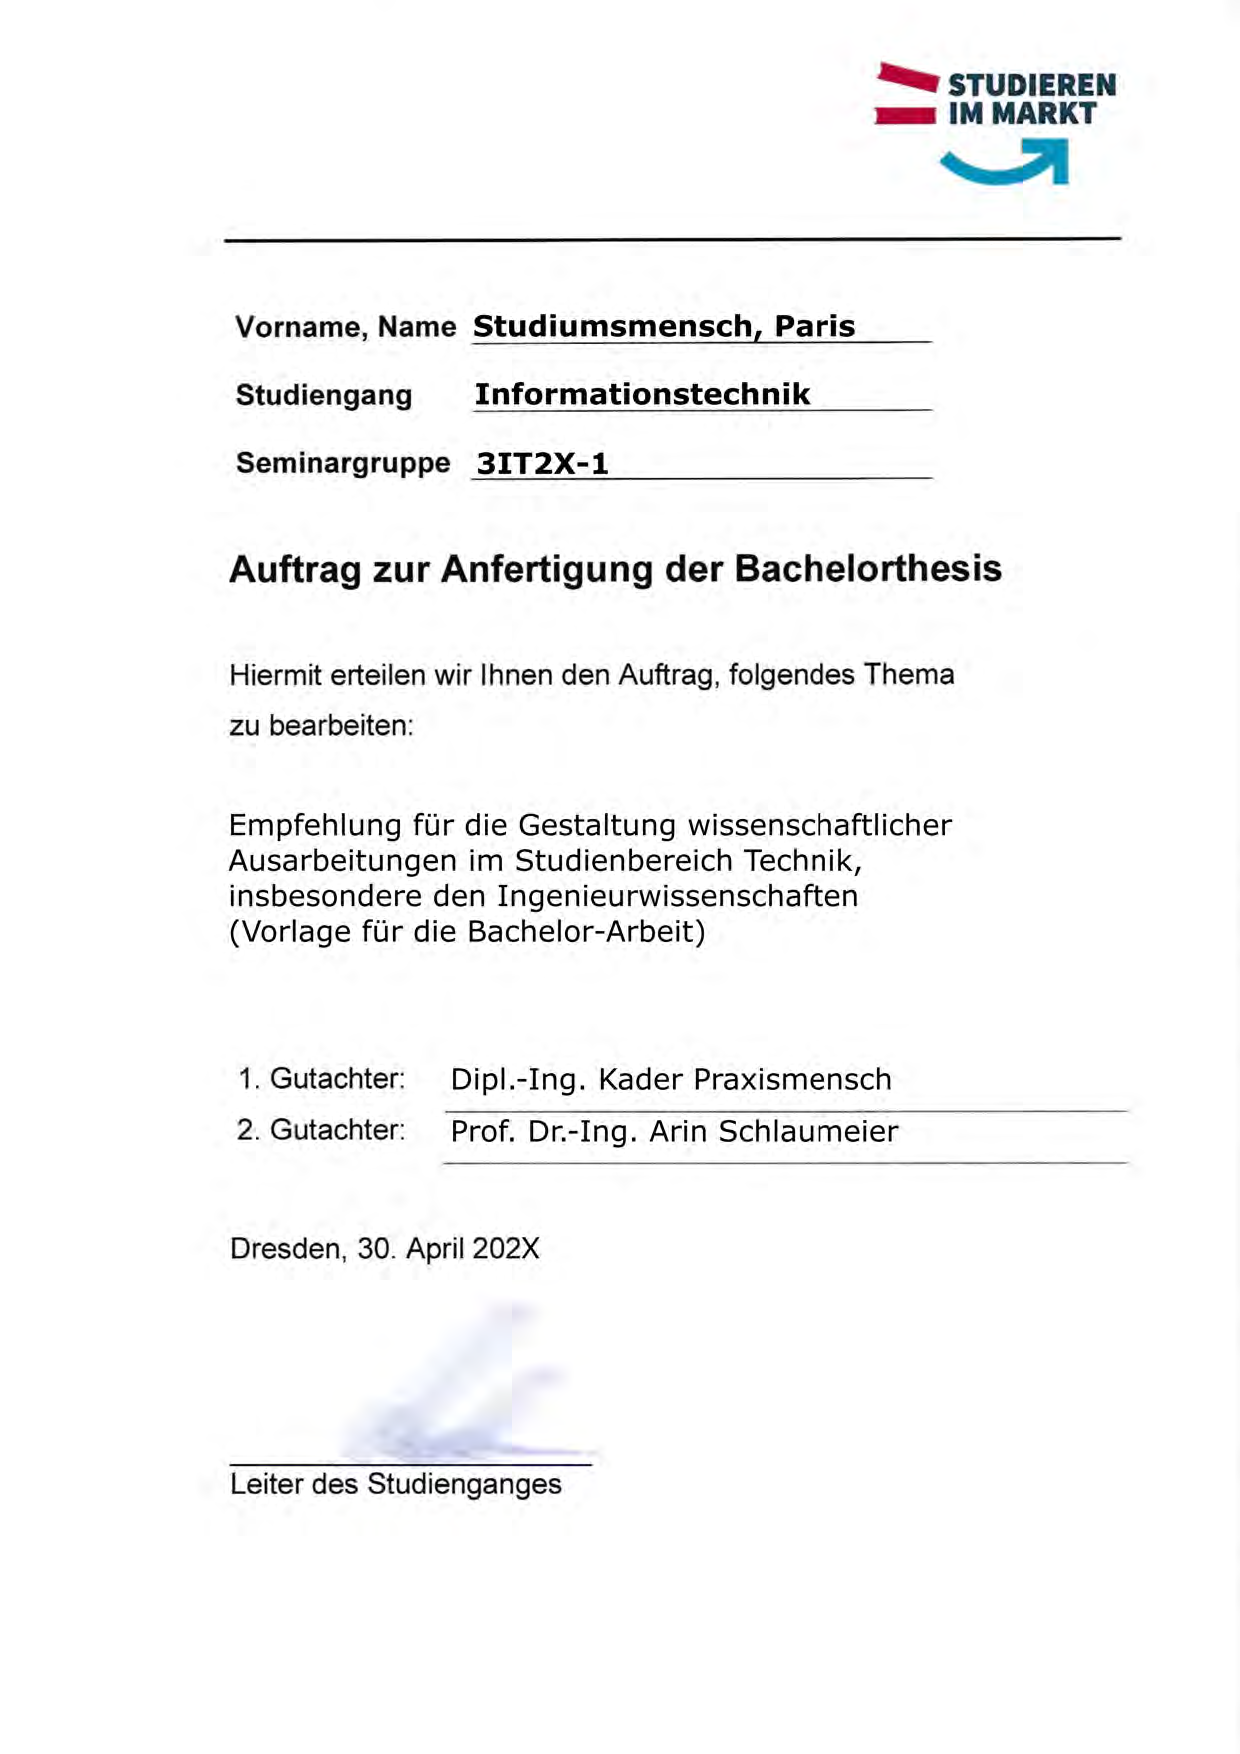
\includepdf[pagecommand={}]{Auftragsblatt.pdf}
%}
{
    \setcounter{page}{\value{page}+1}
}
\include{frontbackmatter/tocLists}

\mainmatter
\pagenumbering{arabic}
\pagestyle{myfancy}
\part{Projektarbeit}
\chapter{Einleitung}\label{chap:Einleitung}
Moderne \gls{ic} bestehen aus einer Vielzahl digitaler und analoger Komponenten, die nach dem Einschalten der Versorgungsspannung einen definierten Anfangszustand benötigen, um fehlerfrei zu funktionieren. Besonders bei komplexeren Systemen, in denen Speicherzellen, Flip-Flops oder digitale Steuerlogik zum Einsatz kommen, ist eine saubere Initialisierung essenziell. Ohne eine gezielte Zurücksetzung können sich undefinierte Betriebszustände einstellen, die die Funktionalität des gesamten Systems gefährden.

Um eine definierte Initialisierung sicherzustellen, wird eine \gls{por}-Schaltung eingesetzt. Diese überwacht die anliegende Versorgungsspannung und erzeugt beim Einschalten ein internes Reset-Signal, welches die relevanten Komponenten des \glspl{ic} in einen vordefinierten Ausgangszustand versetzt. Gleichzeitig stellt die \gls{por}-Schaltung sicher, dass bei Spannungsabfällen oder instabilen Betriebsbedingungen ein Reset ausgelöst wird, um Fehlfunktionen zu verhindern.

Im Rahmen dieser Arbeit wird eine \gls{por}-Schaltung für einen neu entwickelten Chip entworfen. Der Chip beinhaltet sowohl analoge als auch digitale Funktionsblöcke, weshalb separate \gls{por}-Schaltungen für den analogen als auch digitalen Bereich entwickelt werden. Aufgrund unterschiedlicher Versorgungsspannungen und technologischer Anforderungen der beiden Bereiche müssen die Schaltungen an die jeweiligen Bedingungen angepasst werden.

Die Anforderungen an zuverlässige \gls{por}-Schaltungen steigen insbesondere bei modernen Fertigungstechnologien wie dem hier betrachteten 130-nm-CMOS-Prozess, da sich durch Prozessschwankungen, Temperatureinflüsse und Versorgungsspannungsänderungen das Schaltverhalten der Transistoren und passiven Bauelemente erheblich verändern kann. Ziel dieser Arbeit ist die Entwicklung und Verifizierung einer robusten \glspl{por}-Schaltung, die auch unter variierenden \gls{pvt} zuverlässig arbeitet. Dabei liegt der Fokus auf einer stabilen Referenzspannung und einer zuverlässigen Reset-Verzögerung.

Durch Simulationen in der Cadence-Virtuoso-Umgebung wird sichergestellt, dass die entwickelte \gls{por}-Schaltung den vorgegebenen Anforderungen entspricht und eine zuverlässige Initialisierung des analogen und des digitalen Chipbereichs gewährleistet wird.

\chapter{Grundlagen}\label{chap:Grundlagen}

\section{Power-On-Reset-Schaltung}
Bei \glspl{ic} ist es wichtig, dass eine vordefinierte Anfangsbedingung bei Einschalten hergestellt wird. Besonders, wenn in dieser Schaltung Latches oder Speicherkomponenten integriert sind, muss eine  bekannte Anfangsbedingung sichergestellt werden, da sonst fehlerhafte Betriebszustände auftreten können. Sind die Betriebszustände nicht richtig initialisiert worden, kann es zu schwerwiegenden Timing-Problemen und zu Fehlverhalten innerhalb des \glspl{ic} führen. Damit diese Fehlzustände nicht auftreten, wird eine speziell für diesen Zweck konzipierte \gls{por}-Schaltung eingesetzt. Bei dieser wird ein internes Reset-Signal erzeugt, welches Komponenten wie Flip-Flops, Latches, Zähler und Register auf auf vordefinierte Werte zurücksetzt. So wird verhindert, dass sich das System in einem unbekannten Zustand befindet. Sobald der \gls{ic} an eine Versorgungsspannung angeschlossen wird, erkennt die \gls{por}-Schaltung den Spannungsanstieg und hält das Reset-Signal für eine gewisse Zeit ($t_{res}$) aktiv (siehe \autoref{fig:Schwellspannung}),
%\vspace{1.5\baselineskip}
\begin{figure}[H]
    \begin{center}
    \begin{tikzpicture}
        % Achsen
        % \draw[->] (0,0) -- (10,0) node[anchor=north] {s}; % x-Achse
        % \draw[->] (0,0) -- (0,4) node[anchor=east] {V}; % y-Achse

        % Linie
        \draw[thick, blue] 
            (0,0) -- (2,0) % waagerechter Teil von 0 bis 2 Sekunden
            to (5,3) -- ++(5,0);
            % Kreuzungspunkt berechnen
        \coordinate (Kreuzung) at (4,2);

        
        \draw[thick, red] 
            (0,-1) -- ++(6.5,0) -- ++(0,1.5) -- ++(3.5,0);

        % Gestrichelte Linien
        \draw[dashed] 
            (0,2) -- ++ (6,0); % Senkrechte Linie nach unten
        \draw[dashed] 
            (4,3) -- ++(0,-4); % Waagerechte Linie nach rechts
        \draw[dashed] 
            (3,1.75) -- ++(7,0);
            
        % Beschriftungen
        \node[anchor=south, xshift=1cm] at (0,0) {$0\,V$}; % Startpunktbeschriftung
        \node[anchor=south] at (7.5,3) {$5\,V$}; % Endpunktbeschriftung
        \node[] at (-2,0) {\shortstack{Versorgungs- \\spannung}};
        \node[] at (-2,-1) {\shortstack{Reset-Signal}};
        \node[] at (1,2.25) {\shortstack{Schwellspannung $V_H$}};
        \node[] at (9,1.5) {\shortstack{Reset-Spannung $V_L$}};


        \draw[<->, thick, >=stealth] (4,-0.25) -- ++(2.5,0) node[midway, above] {$t_{res}$}; % Pfeil

        
    \end{tikzpicture}        

    \end{center}
    \caption[Schwellspannung]{\\Quelle: Schwellspannung (Eigene Darstellung)}
    \label{fig:Schwellspannung}
\end{figure}
%\vspace{1.5\baselineskip}
damit sich alle auf dem \acrlong{ic} befindlichen Komponenten stabilisieren können. Diese Verzögerung ist außerdem notwendig, um eine zu frühe Freigabe des Reset-Signals zu verhindern, wenn zu Schwankungen oder Spannungsspitzen während der Initialisierungsphase kommt. Nachdem die Verzögerung ($t_{res}$) des Reset-Signals frei gibt, geht das System in den normalen Betriebsmodus über. Die Verzögerungszeit beginnt erst nachdem, eine gewisse Schwellspannung ($V_H$) erreicht ist, damit ein sicherer Betrieb des \glspl{ic} gewährleistet werden kann. Wenn es während des Betriebs zu einem unvorhersehbaren Spannungsabfall kommt,  kann auch das zu einem fehlerhaften Betriebszustand führen, weshalb ein erneuter Reset unverzichtbar ist  (siehe \autoref{fig:Reset-Spannung}). Entscheidend dafür ist, dass die Reset-Spannung ($V_L$) unter der Schwellspannung ($V_H$) für das Reset-Signal liegt. Sobald die Versorgungsspannung unter den Schwellenwert der Reset-Spannung fällt, soll die \gls{por}-Schaltung möglichst ohne Verzögerung den Reset auslösen \cite{9647518}. 
%\vspace{1.5\baselineskip}
\begin{figure}[H]
    \begin{center}
    \begin{tikzpicture}
        % Achsen
        % \draw[->] (0,0) -- (10,0) node[anchor=north] {s}; % x-Achse
        % \draw[->] (0,0) -- (0,4) node[anchor=east] {V}; % y-Achse

        % Linie
        \draw[thick, blue] 
            (0,3) -- (5,3) % waagerechter Teil von 0 bis 2 Sekunden
            to (8,0) -- ++(2,0);
            % Kreuzungspunkt berechnen
        \coordinate (Kreuzung) at (6.25,1.75);

        
        \draw[thick, red] 
            (0,0.5) -- ++(6.25,0) -- ++(0,-1.5) -- ++(3.5,0);

        % Gestrichelte Linien
        \draw[dashed] 
            (Kreuzung) -- ++ (-3.25,0)
            (Kreuzung) -- ++ (3.75,0); % Waagerechte Linien
        \draw[dashed] 
            (Kreuzung) -- ++(0,-1.25)
            (Kreuzung) -- ++(0,1.25); % Senkrechte Linien
        \draw[dashed] (0,2) -- ++ (8,0); % Schwellspannung
            
        % Beschriftungen
        \node[anchor=south, xshift=-1cm] at (10,0) {$0\,V$}; % Startpunktbeschriftung
        \node[anchor=south] at (2.5,3) {$5\,V$}; % Endpunktbeschriftung
        \node[] at (-2,3) {\shortstack{Versorgungs- \\spannung}};
        \node[] at (-2,0.5) {\shortstack{Reset-Signal}};
        \node[] at (1,2.25) {\shortstack{Schwellspannung $V_H$}};
        \node[] at (9,1.5) {\shortstack{Reset-Spannung $V_L$}};
        
    \end{tikzpicture}        

    \end{center}
    \caption[Reset-Spannung]{\\Quelle: Reset-Spannung (Eigene Darstellung)}
    \label{fig:Reset-Spannung}
\end{figure}
%\vspace{1.5\baselineskip}

\section{Differenzverstärker und Komparator}
Ein Komparator (siehe \autoref{fig:Komp}) wird eingesetzt, um zwei analoge Eingangssignale \mbox{($V_{inn}$ und $V_{inp}$)} zu vergleichen und abhängig vom Vergleich einen entsprechendes binäres Ausgangssignal ($V_{out}$) zu liefern. Der Komparatorausgang kann dabei unregelmäßig werden, wenn die Eingangssignale zu stark rauschen. Dieses Rauschen ist ein unerwünschtes Signal, welches nicht mit den Eingangssignal zusammenhängt \cite{7489413}. 
%\vspace{1.5\baselineskip}
\begin{figure}[H]
    \begin{center}
        \begin{circuitikz}[european]
            \ctikzset{tripoles/mos style/arrows}[line width=thick, european]
            % Komparator    
            \draw (0,0) node[op amp] (triangle){}; 
            \draw (triangle) node[above, yshift=27pt] {Komparator};
            \draw (triangle.out) -- ++(1,0) node[above]{$V_{out}$};    
            \draw (triangle.+) -- ++(-1,0) node[above]{$V_{inp}$};
            \draw (triangle.-) -- ++(-1,0) node[above]{$V_{inn}$};

            \draw (7,0.5) node[]{$V_{inp} > V_{inn}$ \hspace{5pt} \textbf{dann} \hspace{5pt} $V_{out} = V_{DD} =$ logische 1};
            \draw (7,-0.5) node[]{$V_{inp} < V_{inn}$ \hspace{5pt} \textbf{dann} \hspace{5pt} $V_{out} = 0 =$ logische 0};

        \end{circuitikz}
    \end{center}
    \caption[Schaltzeichen Komparator]{\\Quelle: Eigene Darstellung Schaltzeichen Komparator in Anlehnung an \cite[S. 909]{CircuitDesigLayoutAndSimulation}}
    \label{fig:Komp}
\end{figure}
% \vspace{1.5\baselineskip}
In einer \gls{por}-Schaltung kann man sich den Komparator als Entscheidungsschaltung vorstellen. Sobald die Betriebsspannung ($V_{inp}$) ein größeres Potential als die Referenzspannung ($V_{inn}$) hat, erhält man am Ausgang des Komparators ($V_{out}$) eine logische 1. Wenn die Betriebsspannung ein niedrigeres Potential aufweist als die Referenzspannung, dann erhält man eine logische 0 am Komparatorausgang \cite{CircuitDesigLayoutAndSimulation}.

\section{Schmitt-Trigger}
Bei nicht Schmitt-getriggerten Bauteilen findet der Schaltvorgang der steigenden und fallenden Flanke immer am gleichen Punkt statt. Bei einem rauschenden Eingangssignal kann der Schwellenwert mehrfach überschritten werden, wodurch eine Mehrfachtaktung oder Oszillation auftreten kann. Dadurch kann es zu einem übermäßigen Stromfluss im gesamten Bauteil kommen. Damit diese Probleme nicht auftreten wird ein Schmitt-Trigger (siehe \autoref{fig:ST_symbol}) verwendet. 
%\vspace{1.5\baselineskip}
\begin{figure}[H]
    \begin{center}
        \begin{circuitikz}[european]
            \ctikzset{tripoles/mos style/arrows}[line width=thick, european]
             % Schmitt-Trigger mit Eingangs- und Ausgangsbezeichnung
            \draw (-4,1) node[schmitt] (schmitt){}; 
            \draw (schmitt) node[above, yshift=27pt] {Schmitt-Trigger};
            
            \draw (schmitt.in) -- ++(-1,0) node[above]{$V_{in}$}; % Eingangsleitung
            \draw (schmitt.out) -- ++(1,0) node[above]{$V_{out}$}; % Ausgangsleitung

            \draw[->, thick] (0,0) -- ++(0,4) node[above]{$V_{out}$}
                coordinate[pos=5/6](VDDy);
                \draw (VDDy) node[left]{\tiny{$V_{DD}$}};
            
            \draw[->, thick] (0,0) -- ++(4,0) node[right]{$V_{in}$}
                coordinate[pos=2/7](VL)
                coordinate[pos=5/7](VH)
                coordinate[pos=10/11](VDD);

            \draw (VDD) -- ++(0,0.1)
                (VDD) -- ++(0,-0.1) node[below]{\tiny{$V_{DD}$}};

            \draw[rounded corners=5pt] (VDDy) -| (VL) -- (VDD);
            \draw[->] (VL) ++(0,2.5) -- ++(0,-2pt);
            \draw[->] (VL) ++(0,0.75) -- ++(0,-2pt);

            \draw[rounded corners=5pt] (VDDy) -| (VH) -- (VDD);
            \draw[->] (VH) ++(0,2.5);
            \draw[->] (VH) ++(0,0.75);
            
            \draw (VH) node[below, xshift=5pt]{\tiny{$V_H$}};
            \draw (VL) node[below, xshift=5pt]{\tiny{$V_L$}};

        \end{circuitikz}
    \end{center}
    \caption[Symbol Schmitt-Trigger]{\\Quelle: Eigene Darstellung Symbol Schmitt-Trigger in Anlehnung an \cite[S. 909]{CircuitDesigLayoutAndSimulation}}
    \label{fig:ST_symbol}
\end{figure}
%\vspace{1.5\baselineskip}
Hauptmerkmal dieses Bauteils ist die Hysterese, welche als Rauschunterdrückung fungiert. Die Schwellenwerte sind so eingestellt, dass die steigende Flanke an einem höheren Punkt ($V_H$) und die fallende Flanke an einem niedrigeren Punkt ($V_L$) schaltet. Die Differenz der beiden Schaltpunkte wird als Hysterese bezeichnet und lässt sich durch das Verhältnis der Transistoren eingestellt werden \cite{CMOS_VLSI_Design}\cite{CircuitDesigLayoutAndSimulation}\cite{texasST}.

\section{Transistoren}
Ein \gls{cmos} ist einer der Schlüsselkomponenten auf heutigen \glspl{ic}. Diese basieren auf der Technologie von \gls{mosfet} und werden als komplementär bezeichnet, da die Kanäle der Transistoren ein komplementäres Paar bilden. \glspl{mosfet} leiten unter bestimmten Bedinungen Strom, da sie aus Halbleitermaterialien bestehen. In der Regel bestehen sie aus Silizium, welches in seiner reinen Form nicht leitfähig ist, und einer Mischung aus Verunreinigungen, wodurch eine Leitfähigkeit erzeugt wird. Abhängig von den Verunreinigungen kann man \gls{mosfet}-Halbleiter in p-Typ und n-Typ unterscheiden. Üblicherweise wird Bor, Gallium und Indium für den p-Typ verwendet und Phosphor, Arsen und Wismut für den n-Typ. Die Halbleiter mit der p-typischen Verunreinigung sind positiv geladen, im Gegensatz dazu besitzen die n-Typen eine negative Ladung. Daraus ergeben sich auch die beiden Haupttypen von \gls{mosfet}-Transistoren \cite{What_is_CMOS}\cite{Göbel2019}. 

In \autoref{fig:nmos_structure} wird der allgemeine Aufbau eines \gls{mosfet}-Transistors mit n-Kanal dargestellt, welcher als \gls{nmos} bezeichnet wird. Das Halbleitergrundmaterial, welches als Substrat bzw. Bulk ($B$) bezeichnet wird, ist p-dotiert und somit gegensätzlich zu der n-Dotierung von Source ($S$) und Drain ($D$). 
\input{figures/Schaltkreise/nmos_structure}
Wenn eine positive Spannung $U_{DS}$ zwischen Source und Drain angelegt wird, sind die beiden pn-Übergänge in Sperrrichtung. Damit ein Strom ($I_{DS}$) zwischen Drain und Source fließen kann, muss eine positive Spannung an das Gate ($G$) angelegt werden. In diesem Fall, lädt sich die Elektrode am Gate positiv auf. Dadurch bildet sich unterhalb der Oxidschicht eine aus Elektronen bestehende Gegenladung. Aufgrund dessen verhält sich der p-Halbleiter wie ein n-dotierter Halbleiter. Die Grenzschicht, die zwischen dem Oxid und dem Halbleiter entsteht, bildet einen Kanal. Dieser verbindet Source und Drain, wodurch der Stromfluss $I_{DS}$ ermöglicht wird \cite{Göbel2019}. 

Die \autoref{fig:MOSFET_Transferkennlinie} zeigt das Symbol eines \gls{nmos}-Transistors und die dazugehörige Transferkennlinie. Diese Kennlinie zeigt den Drainstrom $I_D$ in Abhängigkeit von der Gate-Source-Spannung $V_{GS}$ bei konstantem $V_{DS}$. Wenn $V_{GS}$ eine bestimmte Schwelle $V_{th}$ überschreitet, bildet sich ein leitender Kanal, und Strom kann zwischen Drain und Source fließen.
\begin{figure}
    \centering
    \begin{tikzpicture}
    \ctikzset{tripoles/mos style/arrows}[line width=thick, european]
´         % NMOS-Transistor-Symbol auf der linken Seite
        \begin{scope}[xshift=-3cm] % Verschiebung des Symbols nach links
            \draw (0,2) node[nmos](nmos){};
            \node[above] at (nmos.gate) {$G$}
                (nmos.gate) -- ++(-0.1,0) coordinate(gate)
                node[circle, draw,inner sep=1.5pt]{};
            \node[below, yshift=-5pt] at (nmos.source) {$S$}
                (nmos.source) -- ++(0,-0.1) coordinate(source)
                node[circle, draw,inner sep=1.5pt]{};
            \node[left] at (nmos.drain) {$D$}
                (nmos.drain) -- ++(0,0.1) coordinate(drain)
                node[circle, draw,inner sep=1.5pt]{};

            \draw[->, shorten >=5pt, shorten <=5pt, >=stealth] (drain) to[out=-45,in=45] (source)
                node[xshift=22pt, yshift=25pt]{\footnotesize{$V_{DS}$}};
            \draw[<-, shorten <=5pt, >=stealth] (drain) -- ++ (0,.75) 
                node[right, midway, yshift=5pt]{\footnotesize{$I_D$}};
            \draw[->, shorten >=5pt, shorten <=5pt, >=stealth] (gate) to[out=-90,in=180] (source)
                node[xshift=-25pt]{\footnotesize{$V_{GS}$}};
            \fill[white] (2,1) rectangle (2.975,0);
        \end{scope}

        \begin{axis}[
            xlabel={$V_{GS}$},
            ylabel={$I_D$},
            xmin=0, xmax=4,
            ymin=0, ymax=300,
            xtick=\empty, % Entfernt die Ticks und Beschriftungen der X-Achse
            ytick=\empty,
            width=7cm,
            height=6cm,
            %title={MOSFET Transferkennlinie},
            %title style={yshift=10pt}, % Abstand zwischen Titel und Grafik erhöhen
            %legend pos=north west,
            axis lines=middle, % Achsen in der Mitte mit Pfeilen
            xlabel style={at={(ticklabel* cs:1)}, anchor=north west, xshift=-10pt}, % Beschriftung neben    dem Pfeil
            ylabel style={at={(ticklabel* cs:1)}, anchor=south east, yshift=-10pt}, % Beschriftung neben    dem Pfeil
            minor tick num=0, % Schrittweite entfernen
            minor y tick num=0,
            extra x ticks={1.5}, % Markierung bei V_GS = 1.5
            extra x tick labels={$V_{th}$}, % Beschriftung der Markierung
            extra x tick style={
                grid=none, % Keine Gitterlinie bei der Markierung
                tick pos=left % Tick auf der linken Seite der Achse
            }
        ]
        
        % Beispiel: Quadratische Kennlinie im Sättigungsbereich
        \addplot[
            domain=1.5:4, % V_GS von 1V bis 7V
            samples=100,
            color=blue,
            thick,
        ] {150 * (x - 1.5)^4}; 
        \addplot[
            domain=0:1.5,
            samples=100,
            color=blue,
            thick,
        ] {0};
    
    
        \addplot[
            domain=1.5:4, % V_GS von 1V bis 7V
            samples=100,
            color=red,
            thick,
            style=dashed
        ] {100 * (x - 1.5)^4};
    
        \addplot[
            domain=1.5:4, % V_GS von 1V bis 7V
            samples=100,
            color=red,
            thick,
            style=dashed
        ] {250 * (x - 1.5)^4};
        
        \end{axis}
    \end{tikzpicture}
    \caption[Symbol NMOS-Transistor mit Transferkennlinie]{\\Quelle: Eigene Darstellung Symbol NMOS-Transistor mit Transferkennlinie in Anlehnung an \cite[S. 268]{MicroelectronicCircuits}}
    \label{fig:MOSFET_Transferkennlinie}
\end{figure}
Für die Berechnung des Drainstroms im Sättigungsbereich (wenn $V_{DS} \geq V_{GS} - V_{TH}$) wird diese Formel verwendet: 
\begin{equation}
    I_D = \beta (V_{GS} - V_{TH})^2
\end{equation}
\begin{equation}
    \beta = \alpha \frac{W}{L}
\end{equation}
\begin{equation}
    \alpha = \frac{1}{2} \mu_n C_{ox}
\end{equation}
Die Prozessparameter $\mu_n$ und $C_{ox}$ geben die Beweglichkeit der Ladungsträger und die Oxidkapazität pro Flächeneinheit an und lassen sich während des Schaltungsentwurfs nicht beeinflussen. Durch gezielte Anpassung der Kanalbreite ($W$) und Kanallänge ($L$) können die elektrischen Eigenschaften der \gls{mosfet}-Transistoren beeinflusst werden. Eine größere Kanalbreite ($W$) führt zu einer gesteigerten Stromfähigkeit des Transistors, da auf einem breiteren Kanal mehr Ladungsträger transportiert werden können. Dies führt außerdem zu einem gesteigerten Drainstorm ($I_D$), wodurch die Schaltgeschwindigkeit verbessert wird. Allerdings steigt dadurch eine größere Kanalbreite auch der Energieverbrauch. Die Kanallänge ($L$) hingegen beeinflusst den Widerstand des Kanals. Eine kürzere Kanallänge reduziert diesen Widerstand und erhöht die Geschwindigkeit des Transistors. Dadurch können aber kurz Kanal-Effekte auftreten, die zu erhöhten Leckströmen und Instabilität führen können. Aus diesen Gründen muss ein Kompromiss zwischen Leistung, Energieverbrauch und Stabilität gefunden werden, weshalb eine gezielte Anpassung des $W/L$-Verhältnis notwendig ist \cite{MicroelectronicCircuits}.
    
Der Aufbau eines p-Kanal \gls{mosfet} ist grundsätzlich der gleiche wie beim \gls{nmos}, jedoch ist die Dotierung umgekehrt (siehe \autoref{fig:pmos_structure}). Das Substrat ist n-dotiert und die \mbox{Source-/Draingebiete} p-dotiert, was eine Umkehr der Vorzeichen zur Folge hat. 
%\vspace{1.5\baselineskip}
\begin{figure}[H]
    \begin{center}
        \begin{tikzpicture}
            % N-Type Substrate
            \fill[lightgray] (-4,1) rectangle (4,-1);
            \node at (2.5,-.7) {\textbf{n-Halbleiter}};
            
            % P+ regions
            \fill[gray]
                (-3,1) -- (-1.5,1) -- 
                ++(0,-0.83) arc[start angle=0, end angle=-90, radius=5pt] -- 
                ++(-1.15,0) arc[start angle=-90, end angle=-180, radius=5pt] -- 
                cycle;
            \node at (-2.25,0.5) {\textbf{p}};
            \fill[gray]
                (1.5,1) -- (3,1) -- 
                ++(0,-0.83) arc[start angle=0, end angle=-90, radius=5pt] -- 
                ++(-1.15,0) arc[start angle=-90, end angle=-180, radius=5pt] -- 
                cycle;
            \node at (2.25,0.5) {\textbf{p}};

            % Gate
            \fill[gray]
                (-1.5,1.75) rectangle (1.5,1.25);
            \node at (0,1.5) {{Metall}};
            \draw (-1.5,1.25) rectangle (1.5,1)
                node at (0,1.125) {\tiny{Oxid}};
            \draw (0,1.75) -- ++(0,0.5)   
                node[circle, draw,inner sep=1.5pt] at (0,2.325){}
                    node[right]{$G$};

            % Source 
            \draw (-2.25,1) -- ++(0,0.5)   
                node[circle, draw,inner sep=1.5pt] at (-2.25,1.575){}
                    node[right]{$S$};
                    
            % Drain 
            \draw (2.25,1) -- ++(0,0.5)   
                node[circle, draw,inner sep=1.5pt] at (2.25,1.575){}
                    node[right]{$D$};

            % Bulk
            \draw (0,-1) -- ++(0,-0.5)   
                node[circle, draw,inner sep=1.5pt] at (0,-1.575){}
                    node[right]{$B$};
                    
        \end{tikzpicture}
    \end{center}
    \caption[Struktur PMOS-Transistor]{\\Quelle: Eigene Darstellung Struktur PMOS-Transistor in Anlehnung an \cite[S. 107]{Göbel2019}}
    \label{fig:pmos_structure}
\end{figure}
% \vspace{1.5\baselineskip}
Wenn beispielsweise 0 V an Gate und Drain sowie 5~V an Source und Bulk, ergibt sich eine negative Gate-Source-Spannung $U_{GS}$ von -5 V. Da $U_{DS}$ auch eine negative Spannung hat, fließt ein negative Drain-Source Strom $I_{DS}$. Dabei ist zu beachten, dass sowohl für den \gls{nmos} als auch für den \gls{pmos} eine gewisse Schwellspannung überschritten werden muss, damit sich der Kanal zwischen Source und Drain bilden kann~\cite{Göbel2019}.  

Native Transistoren, zeichnen sich durch eine sehr geringe Schwellspannung nahe Null aus. Diese Eigenschaft unterscheidet sie grundlegend von herkömmlichen Transistoren, die eine bestimmte Gate-Source-Spannung benötigen, um Strom zu leiten. Damit dies möglich ist, wird die Dotierung im Kanalbereich angepasst. Bei einem \gls{nmos}-Transistor ist der Kanal leicht n-dotiert, anstatt p-dotiert. Aufgrund dessen ist ein Native Transistor bereits ohne angelegte Gate-Source-Spannung leitfähig, was ihn besonders für Anwendungen in einer Low-Power-Schaltung nützlich macht \cite{Evolution}.

\section{Stromspiegel}
Ein Stromspiegel (siehe \autoref{fig:current_mirror}) ist eine grundlegende Schaltung im analogen \gls{ic}-Entwurf, die dazu dient, einen definierten Strom ($I_{in}$) von einem Referenzzweig auf einen Ausgangszweig ($I_{out}$) zu übertragen.
%\vspace{1.5\baselineskip}
\begin{figure}[H]
    \begin{center}
        \begin{circuitikz}[european]
            \ctikzset{tripoles/mos style/arrows}[line width=thick, european]
            
            % Transistoren 
            \draw (-2,0) node[nmos, yscale=-1, rotate=180](nmosL){}
                node at (nmosL.center) [anchor=center, xshift=-10pt]{$N_0$};
            \draw (2,0) node[nmos](nmosR){$N_1$};

            \draw (nmosL.gate) -- (nmosR.gate)
                coordinate[pos=0.5](gate_cross)
                (gate_cross) node[circle, fill, inner sep=1.5pt]{};

            \draw (nmosL.drain) -- ++(0,0.25) 
                coordinate(left_cross)
                node[circle, fill, inner sep=1.5pt]{};

            \draw (left_cross) -| (gate_cross);

            \draw (left_cross) -- ++(0,1.25);
            \draw (nmosR.drain) -- ++(0,1.5);

            % Ground 
            \draw (nmosL.source) -- ++ (0,-0.5) -- ++ (2,0)
                node[circle, fill, inner sep=1.5pt]{};
            \draw (nmosR.source) -- ++ (0,-0.5) -- ++ (-2,0)
                coordinate(ground);
            \draw (ground) -- ++(0,-.25) node[sground]{}
                node[right, xshift=5pt, yshift=-7pt]{Gnd};

            % Ströme
            \draw[->, thick, >=stealth] (-2.25,2) -- ++(0,-.75)
                node[left, yshift=10pt]{$I_{in}$};
            \draw[->, thick, >=stealth] (2.25,2) -- ++(0,-.75)
                node[right, yshift=10pt]{$I_{out}$};

        \end{circuitikz}
    \end{center}
    \caption[Aufbau Stromspiegel]{\\Quelle: Eigene Darstellung Aufbau Stromspiegel in Anlehnung an \cite[S. 512]{MicroelectronicCircuits}}
    \label{fig:current_mirror}
\end{figure}
Dadurch ist der Stromspiegel eine wichtige Komponente im analogen Schaltungsentwurf, insbesondere für Referenzstromquellen und Differenzverstärker. Ein typischer Stromspiegel besteht aus zwei \gls{mosfet}-Transistoren, die so verbunden sind, dass einer als Referenztransistor ($N_0$) und der andere als Lasttransistor ($N1$) agieren. Da beide Transistoren die gleiche Gate-Source-Spannung ($V_{GS}$) besitzen, ist auch der Drainstrom ($I_D$) identisch. Haben die Transistoren $N_1$ und $N_2$ das gleiche $W/L$-Verhältnis, so wird der Strom $1:1$ gespiegelt ($I_{out} = I_{in}$). Der Ausgangsstrom ($I_{out}$) wird durch das $W/L$-Verhältnis der Transistoren beeinflusst und kann durch folgende Gleichung berechnet werden: 
\begin{equation}
    \frac{I_{in}}{I_{out}} = \frac{(W/L)_{N_0}}{(W/L)_{N_1}} \Rightarrow I_{out} = I_{in} \frac{(W/L)_{N_1}}{(W/L)_{N_0}}
\end{equation}dia
\chapter{Funktionsgruppen der Power-on-Reset-Schaltung}\label{chap:Schaltung}
Um eine zuverlässige Initialisierung des Chips zu erfüllen, wurde eine aus mehreren funktionalen Blöcken bestehende \gls{por}-Schaltung aufgebaut. Jede dieser Funktionsgruppen übernimmt eine spezifische Aufgabe innerhalb der Gesamtschaltung und trägt zur korrekten Erzeugung und Freigabe des Reset-Signals bei. Die wesentlichen Funktionsblöcke umfassen die Generierung einer Referenzspannung, eine zuverlässige Vergleichsschaltung, eine zeitgesteuerte Verzögerung zur sicheren Initialisierung sowie eine Schmitt-Trigger-Stufe zur Verbesserung der Störfestigkeit. 

Durch die modulare Aufteilung kann jeder dieser Blöcke gezielt auf die Anforderungen des analogen oder digitalen Teils des Chips angepasst werden. In den folgenden Abschnitten werden diese detailliert beschrieben und ihr Beitrag zur Gesamtschaltung erläutert (Kapitel 3.1 - 3.4). Anschließend wird dargelegt, welche Anpassungen für den Komparator des Digitalteils notwendig waren (Kapitel 3.5). 


\section{Komparator}
Ein entscheidendes Bauteil der \gls{por}-Schaltung ist der Komparator, da dieser bestimmt, wann das Reset-Signal aktiviert oder deaktiviert wird. Für die Realisierung des Komparators (siehe \autoref{fig:komparator}), werden \gls{cmos}-Transistoren verwendet. Hauptbestandteil dieser Schaltung ist das differenzielle Paar \gls{nmos}-Transistoren ($N_1$ und $N_2$), die an ihren Gates die Eingangssignale ($V_{inn}$ und $V_{inp}$) vergleichen. Dieses Paar bestimmt, welcher Transistor mehr Strom leitet, in Abhängigkeit von der Spannungsdifferenz zwischen $V_{inn}$ und $V_{inp}$~\cite{DesignOfAnalogCMOSIntegratedCircuits}. Der darüber liegende Stromspiegel, bestehend aus zwei \gls{pmos}-Transistoren ($P_0$ und $P_1$) und sorgt dafür, dass der gleiche Strom durch beide Seiten des Differenzverstärkers fließt. Damit wird sichergestellt, dass die Schaltung symmetrisch arbeitet. Für eine konstante Stromversorgung ist der \gls{nmos}-Transistor $N_3$ zuständig, der sich unter dem Differenzpaar $N_1$ und $N_2$ befindet \cite{ADofIntegratedCircuits}. 
%\vspace{1.5\baselineskip}
\begin{figure}[H]
    \begin{center}
        \begin{circuitikz}
            \ctikzset{tripoles/mos style/arrows}[line width=thick]
            \draw % Transformatoren 
            (3,0) node[pmos, emptycircle](pmosR){$P_2$}
            (-3,0) node[pmos, emptycircle, yscale=-1, rotate=180](pmosL){} 
                node at (pmosL.center) [anchor=center, xshift=-10pt] {$P_1$}
            
            (-3,-3) node[nmos, emptycircle](nmosL){$N_1$}
            (3,-3) node[nmos, emptycircle, yscale=-1, rotate=180](nmosR){}
                node at (nmosR.center) [anchor=center, xshift=-10pt] {$N_2$}
    
            (0,-5) node[nmos, emptycircle](nmos){$N_3$}
    
            % Verbindung zwischen Transformatoren
            (pmosR.drain) -- (nmosR.drain){}
                coordinate[pos=0.5](crosspointRR) % Mittelpunk zwischen pmosR und nmosR
            (pmosL.drain) -- (nmosL.drain){}
                coordinate[pos=0.5](crosspointLL) % Mittelpunk zwischen pmosL und nmosL
            (nmosL.source) -- ++(0,-0.25) -- ++(3,0)
            (nmosR.source) -- ++(0,-0.25) -- ++(-3,0) coordinate(Ibias)
                (Ibias) node[circle, fill, inner sep=1.5pt]{}
            (Ibias) -- (nmos.drain)
            
            (pmosL.source) -- ++(0,0.5) coordinate (tmp1) 
                -- ++(6,0) coordinate (tmp2) % rechte obere Koordinate
                -- (pmosR.source) coordinate (tmp3)
                (tmp1) -- (tmp2)
                    coordinate[pos=0.5](crosspointVdd)
                        (crosspointVdd) -- ++(0,0.5) coordinate(VDD)
                            node[above] {$V_{DD}$} % Text zwische Koordinate 1 und 2
                        (VDD) -- ++(-0.5,0)
                        (VDD) -- ++(0.5,0)
    
            (pmosL.gate) -- (pmosR.gate){}
                coordinate[pos=0.5](crosspointLR) % Mittelpunk zwischen pmosL und pmosR
    
            % Knoten und Verbindungen 
            (crosspointLL) node[circle, fill, inner sep=1.5pt]{} % Knoten links
            (crosspointLR) node[circle, fill, inner sep=1.5pt]{} % Knoten mitte
            (crosspointLL) -| (crosspointLR){} % Verbindung zwischen linken und mittleren Knoten
            (crosspointRR) node[circle, fill, inner sep=1.5pt]{}
                (crosspointRR) -- ++(1.5,0)
                    node[pos=1, above right, xshift=-15pt]{$V_{out}$}
            
            % Verbindung nmos.gate
            (nmosL.gate) -- (-4.5,-3)
                node[pos=0, above left]{$V_{inn}$}
            (nmosR.gate) -- (4.5,-3)
                node[pos=0, above right]{$V_{inp}$}
            (nmos.gate) -- (-1.5,-5)
                node[pos=0, above left]{$V_{ref}$}
    
            % Ground
            (nmos.source) 
                node [sground]{}
                node[right, xshift=5pt, yshift=-5pt]{Gnd}
            ;
    
        \end{circuitikz}
    \end{center}
    \caption[Aufbau Komparator für analogen Teil]{\\Quelle: Aufbau Komparator für analogen Teil (eigene Darstellung)}
    \label{fig:komparator}
\end{figure}
% \vspace{1.5\baselineskip}
Wenn die Spannung $V_{inn}$, die am Gate $N_1$ anliegt, größer ist als die Spannung $N_2$, dann wird $V_{inn}$ nach oben über den Stromspiegel zu $V_{out}$ geleitet. Ist $V_{inp}$ größer als $V_{inn}$, fließt der Strom direkt zu $V_{out}$ und nicht über den Stromspiegel. 

\section{Referenzspannung}
Damit ein zuverlässiges Reset-Signal generiert werden kann, wird eine Referenzspannung ($V_{ref}$) benötigt, die als Vergleichswert für die Schaltpunkte des Komparators dient. Für die Generierung von $V_{ref}$ sowie den Schaltpunkten des Komparators wird die Schaltung~(siehe \autoref{fig:Vref_old}) entworfen, welche sich wiederum in einzelne Funktionsblöcke unterteilen lässt. Der erste Funktionsblock ist die Generierung der Referenzspannung mittels Widerstandsteiler. Dieser besteht aus dem Widerstand~($R_0$) und \gls{nmos}-Transistor~($N_0$), wobei der Wert von $V_{ref}$ abhängig von der Dimensionierung von $R_0$ und $N_0$ ist. Ein weiterer entscheidender Bestandteil der Schaltung ist der Spannungsteiler, bestehend aus den Widerständen $R_1$,$R_2$ und $R_3$. Durch die gezielte Wahl der Widerstandswerte lassen sich die Schaltschwellen der \gls{cmos}-Transistoren festlegen, sodass diese bei bestimmten Spannungswerten umschalten. 
%\vspace{1.5\baselineskip}
\begin{figure}[H]
    \begin{center}
        \begin{circuitikz}[european]
            \ctikzset{tripoles/mos style/arrows}[line width=thick, european]
            % Widerstand
            \draw (-3,5) coordinate(resistor-begin) to[resistor, l={$R_0$}] (-3,0.5) coordinate(resistor-end);

            \draw (resistor-begin) node[circle, fill, inner sep=1.5pt]{};
            
            % NMOS Transistor
            \draw (-3,-0.5) node[nmos, anchor=drain] (nmosL) {$N_0$};

            % Verbindung von Drain des NMOS mit Widerstand
            \draw (resistor-end) -- (nmosL.drain);
            \draw (nmosL.gate) -- ++(-0.25,0) |- (resistor-end)
                node[circle, fill, inner sep=1.5pt]{}
                node[above, midway]{$V_{ref}$};
            %
            %*************************************************************************
            %
            % Widerstand R
            \draw (0,5) coordinate (resistor-begin1) to[resistor, l={$R_1$}] (0,2) coordinate (resistor-end1);
            \draw (0,2) coordinate (resistor-begin2) to[resistor, l={$R_2$}] (0,-1) coordinate (resistor-end2);
            \draw (0,-1) coordinate (resistor-begin3) to[resistor, l={$R_3$}] (0,-4) coordinate (resistor-end3);

            % NMOSR 
            \draw (3,2) node[nmos, rotate=270] (nmosR1) {}
                node at (nmosR1.center) [anchor=center, yshift=-10pt] {$N_1$}
                (nmosR1.source) -- (resistor-end1) % Verbinung zu Wiederständen 
                node[circle, fill, inner sep=1.5pt]{}; % Punkt am Ende der Verbindung 
            \draw (3,-1) node[nmos, rotate=270] (nmosR2) {}
                node at (nmosR2.center) [anchor=center, yshift=-10pt] {$N_2$}
                (nmosR2.source) -- (resistor-end2)
                node[circle, fill, inner sep=1.5pt]{};

            % NMOS Drain Verbindung
            \draw (nmosR1.drain) -- ++ (0.25,0) % horizontal nach rechts
                -- ++ (0,-3) coordinate (comp) % vertikale Linie 
                node[circle, fill, inner sep=1.5pt]{};

            \draw (nmosR1.gate) -- ++(0,0.25) -- ++(-0.75,0) 
                node[above, midway]{$V_{res}$};
            \draw (nmosR2.gate) -- ++(0,0.25) -- ++(-0.75,0)
                node[above, midway]{$V_{res0}$};

            % Dreieck am Ende von Vcomp
            \draw (6.75,-0.51) node[op amp] (triangle){}
                (triangle.+) -- (nmosR2.drain);
            \draw (triangle) node[above, yshift=27pt] {Komparator};  

            \draw (triangle.-) -- ++(-0.5,0) node[above]{$V_{ref}$};

            % Verbindung Ground
            \draw (nmosL.source) |- (resistor-end3)
                node[circle, fill, inner sep=1.5pt]{}
                -- ++(0,-0.25) node[sground]{}
                node[right, xshift=5pt, yshift=-5pt]{Gnd};     

            % Verbindung VDD
            \draw (resistor-begin1) -- ++(-3.73,0)
                node[above] {$V_{DD}$};

            % Arrow 
            \draw[->, thick, shorten >=10pt, shorten <=10pt, >=stealth] (resistor-end1) to[out=225,in=135] (resistor-end3)
                node[midway, left, xshift=-35pt, yshift=-10pt]{$V_{DD1}$};
                
            \draw[->, thick, shorten >=10pt, shorten <=10pt, >=stealth] (resistor-end2) to[out=-25,in=25] (resistor-end3)
                node[right,xshift=20pt, yshift=50pt]{$V_{DD2}$};
        \end{circuitikz}
    \end{center}
    \caption[Generierung des Referenzstrom durch Widerstand]{\\Quelle: Generierung des Referenzstrom durch Widerstand (Eigene Darstellung)}
    \label{fig:Vref_old}
\end{figure}
%\vspace{1.5\baselineskip}
Die Transistoren $N_1$ und $N_2$ werden mit den Signalen $V_{res}$ und $V_{res0}$ gesteuert. Außerdem verbinden $N_1$ und $N_2$ die Spannung $V_{DD1}$ und $V_{DD2}$ mit dem positiven Eingang des Komparators. Diese \gls{cmos}-Schalter sorgen somit für eine gezielte Modifikation der Vergleichsspannung, die dem Komparator zugeführt wird. Der Komparatorausgang wird durch eine nachgestellte Inverter-Kette verarbeitet, die als Buffer dienen und die Ausgangssignale $V_{res}$ und $V_{res0}$ zur Verfügung stellen. Somit wird bei inaktiven Reset-Signal ($V_{comp} = 0$) die höhere Spannung ($V_{DD1}$) als Vergleichsspannung verwendet, wodurch die höhere Schwellspannung $V_H$ (siehe \autoref{fig:Schwellspannung}) erzeugt wird. Im Gegensatz dazu wird bei einem aktiven Resest-Signal ($V_{comp} = 1$) die niedrigere Spannung $V_{DD2}$ verwendet, sodass eine geringere Reset-Spannung ($V_L$) (siehe \autoref{fig:Reset-Spannung}) realisiert wird.
\cite{DesignOfAnalogCMOSIntegratedCircuits}\cite{MicroelectronicCircuits}.

\section{Verzögerung des Reset}
Bei einer \gls{por}-Schaltung muss sichergestellt werden, dass der Reset-Zustand so lange aufrechterhalten wird, bis die Versorgungsspannung stabil ist. Gleichzeitig muss das System bei einem plötzlichen Spannungsabfall schnell in den Reset-Zustand zurückkehren, um Fehlfunktionen zu vermeiden. In diesem Schaltungsteil (siehe \autoref{fig:Delay}) der \gls{por}-Schaltung, wird die verzögerte Aktivierung beim Hochfahren als auch eine schnelle Reaktion beim Abfallen der Versorgungsspannung realisiert.
%\vspace{1.5\baselineskip}
\begin{figure}[H]
    \begin{center}
        \begin{circuitikz}[european]
            \ctikzset{tripoles/mos style/arrows}[line width=thick, european]
            
            % Transistoren links
            \draw (-4,0) node[pmos, emptycircle, yscale=-1, rotate=180](pmosL){}
                node at (pmosL.center) [anchor=center, xshift=-10pt]{$P_0$}
                (-4,-3) node[nmos](nmosL){$N_0$};
                
            % Transistoren rechts
            \draw (0,0) node[pmos, emptycircle](pmosR1){$P_1$}
                (0,-3) node[pmos, emptycircle](pmosR2){$P_2$}
                (0,-6) node[nmos](nmosR){$N_1$};
                
            % Verbindungen Transistroen links
            \draw (pmosL.drain) -- (nmosL.drain) 
                coordinate[pos=0.5](crosspointLL) % Mitte links
                (crosspointLL) node[circle, fill, inner sep=1.5pt]{}; % Verzweigung links 
                
            % Verbindung pmos gate
            \draw (pmosL.gate) -- (pmosR1.gate)
                coordinate[pos=0.5](crosspointPP)
                (crosspointPP) node[circle, fill, inner sep=1.5pt]{};
            \draw (nmosL.gate) -- ++(-.5,0)
                node[above]{$V_{gate}$}
                (nmosL.source) node[sground]{}
                node[right, xshift=5pt, yshift=-5pt]{Gnd};
                
            % Kurzschluss 
            \draw (crosspointLL) -| (crosspointPP);

            % VDD
            \draw (pmosL.source) -- ++(0,0.5) 
                node[circle, fill, inner sep=1.5pt]{};
            \draw (pmosR1.source) -- ++(0,0.5) -- ++(-5.475,0) 
                node[above]{$V_{DD}$};
                
                
            % Verbindungen rechts    
            \draw (pmosR1.drain) -- (pmosR2.source)
                (pmosR2.drain) -- (nmosR.drain)
                    coordinate[pos=0.5](crosspointRR) % Mittelpunkte rechts
                    (crosspointRR) node[circle, fill, inner sep=1.5pt]{}
                (nmosR.source) -- ++(2,0) coordinate[](nmosC)
                (nmosC) node[circle, fill, inner sep=1.5pt]{};
                
            % Gate rechts
            \draw (pmosR2.gate) -- ++(-0.5,0)
                    -- ++(0,-3) node[circle, fill, inner sep=1.5pt]{}
                (nmosR.gate) -- ++(-4.5,0) 
                    node[above]{$V_{comp}$};
                    
            % Kondensator 
            \draw (2,-4.5) node[circle, fill, inner sep=1.5pt]{}
                (2,-4.5) to[C, l={$C$}] (2,-6.5) -- (nmosC)
                (nmosC) -- ++(0,-0.25) node[sground]{}
                node[right, xshift=5pt, yshift=-5pt]{Gnd};
            \draw (crosspointRR) -- ++(4,0)
                node[above]{$V_{schmitt}$};
                
        \end{circuitikz}
    \end{center}
    \caption[Verzögerungselement]{\\Quelle: Verzögerungselement (eigene Darstellung)}
    \label{fig:Delay}
\end{figure}
% \vspace{1.5\baselineskip}
Zentraler Bestandteil dieses Schaltungsabschnitts ist der Stromspiegel, der aus zwei gekoppelten \gls{pmos}-Transistoren besteht. Der linke Transistor $P_0$ arbeitet als Referenzzweig, $P_1$ bildet den gespiegelten Zweig, der $^1/_5$ des Stroms führt, da die Kanalbreiten der \gls{pmos}-Transistoren ein Verhältnis von ${W_{P_0}}/{W_{P_1}} = \frac{1}{5}$ haben. Dieser Strom sorgt für die Ladung des Kondensators $C$ \cite{CircuitDesigLayoutAndSimulation}. Beim Anlegen der Versorgungsspannung ist der Kondensator zunächst ungeladen, und $V_{schmitt}$ bleibt auf 0. Der durch den Stromspiegel gelieferte Strom lädt $C$ langsam auf, weshalb die Spannungsänderung an $V_{schmitt}$ nur verzögert auftritt, was durch 
\begin{equation}
    i = C \frac{du}{dt}
\end{equation}
berechnet werden kann. Um den Ladevorgang zu verlängern, kann $C$ größer oder $I$ kleiner gewählt werden \cite{MicroelectronicCircuits}\cite{DesignOfAnalogCMOSIntegratedCircuits}. Wenn es einen Abfall von $V_{DD}$ gibt, soll so schnell wie möglich der Reset-Zustand wiederhergestellt werden. In diesem Fall wird der $N_1$ sofort leitend, wodurch sich der Kondenstor direkt über diesen Transistor nach Masse entlädt. Durch die hohe Elektronenbeweglichkeit im \gls{nmos}-Kanal wird $C$ im Vergleich zur Ladezeit sehr schnell entladen. Somit wird das Reset-Signal sofort ausgelöst und das System in einen definierten Startzustand zurückgesetzt \cite{ElectronicDevices}. 

\section{Schmitt-Trigger}
Ein Schmitt-Trigger ist eine spezielle Art von Komparator mit Hysterese, dieser erzeugt ein stabiles Ausgangssignal, indem kleinere Spannungsschwankungen oder Rauschen am Eingang ignoriert werden. Die Schaltung aus \autoref{fig:schmitt-trigger} besteht aus einer Kombination aus \gls{pmos}- und \gls{nmos}-Transistoren, die in einer invertierten Struktur miteinander verbunden sind. 
%\vspace{1.5\baselineskip}
\begin{figure}[H]
    \begin{center}
        \begin{circuitikz}
            \ctikzset{tripoles/mos style/arrows}[line width=thick]
            \draw % Transformatoren 
            (0,2.5) node[pmos, emptycircle](pmos1){$P_0$}
            (3,0.95) node[pmos, emptycircle](pmos2){$P_2$}
            (0,0) node[pmos, emptycircle](pmos3){$P_1$} 
            (0,-2) node[nmos](nmos1){$N_0$}
            (3,-2.95) node[nmos](nmos2){$N_2$}
            (0,-4.5) node[nmos](nmos3){$N_1$};
        
            %Verbindung zwischen Transistoren
            \draw (pmos1.drain) -- (pmos3.source); % Verbindung von pmos1 zu pmos3 (senkrecht)
            \draw (pmos2.source) -- (pmos1.drain) % Verbindung zu pmos2 
                node[circle, fill, inner sep=1.5pt] {}; % Punkt an Verbindung
            \draw (pmos3.drain) -- (nmos1.drain); % Verbindung von pmos3 zu nmos1 
            \draw (nmos1.source) -- (nmos3.drain); % Verbindung von nmos1 zu nmos3
            \draw (nmos2.source) -- (nmos3.drain) % Verbindung zu noms2 
                node[circle, fill, inner sep=1.5pt] {};
            \draw (nmos3.source) 
                node[sground] {}
                node[right, xshift=5pt, yshift=-5pt]{Gnd};
            \draw (pmos2.drain)
                node[sground,] {}
                node[right, xshift=5pt, yshift=-5pt]{Gnd}; % Ground an pmos2
            \draw (pmos2.gate) -- (nmos2.gate) 
                coordinate[pos=0.5](crosspoint); % Mittelpunkt der Verbindung 
            
            % Vin                           
            \draw (-2.5,-1) -- (-1.5,-1) coordinate (Vin)% Vin Linie (zu Gates)
                node[pos=0, above left, xshift=10pt] {$V_{in}$} % Beschriftung oberhalb der Linie
                node [circle, fill, inner sep=1.5pt] {};

            %Vin connections 
            \draw (5,-1) -- (0,-1) % Vout Linie
                node [pos=0, above right, xshift=-25pt] {$V_{out}$}
                node [circle, fill, inner sep=1.5pt] {};
            \draw (crosspoint) node[circle, fill, inner sep=1.5pt] {}; % Punkt an Kreuzung
            \draw % Verbindung der Gates
                (pmos1.gate) -- ++(-0.5,0) -- (Vin);
            \draw % Verbindung der Gates
                (nmos3.gate) -- ++(-0.5,0) -- (Vin);
            \draw % Verbindung der Gates
                (pmos3.gate) -- ++(-0.5,0) 
                node[circle, fill, inner sep=1.5pt] {};
            \draw % Verbindung der Gates
                (nmos1.gate) -- ++(-0.5,0) 
                node[circle, fill, inner sep=1.5pt] {};    

            % VDD 
            \draw (-0.5,3.5) -- (0.5,3.5) % VDD an pmos1
                node[midway, above] {$V_{DD}$} % Beschriftung oberhalb der Linie
                (0,3.5) -- (pmos1.source);
            \draw (2.5,-1.95) -- (3.5,-1.95) % VDD an nmos2
                node[midway, above] {$V_{DD}$} % Beschriftung oberhalb der Linie
                (3,-1.95) -- (nmos2.drain); 
                
        \end{circuitikz}
    \end{center}
    \caption[Aufbau Schmitt-Trigger]{\\Quelle: Eigene Darstellung Aufbau Schmitt-Trigger in Anlehnung an \cite[S. 524]{CircuitDesigLayoutAndSimulation}}
    \label{fig:schmitt-trigger}
\end{figure}
%\vspace{1.5\baselineskip}
Die Schaltschwellen des Komparators $V_H$ und $V_L$ (siehe \autoref{fig:ST_symbol}) können durch die Dimensionierung der Länge ($L$) und Weite ($W$) der Transistroen eingestellt werden \cite{CircuitDesigLayoutAndSimulation}\cite{S-Trigger_design}\cite{LowPowerS-Trigger}.  

\section{Gesamte PoR-Schaltung}
Nach einem Test der einzelnen Funktionsblöcke auf ihre jeweilige Funktionalität, wurden diese Blöcke zu einem Gesamtsystem (siehe \ref{fig:PoR_complete}) zusammengesetzt. Der erste vollständige Aufbau der \gls{por}-Schaltung erfolgte für den analogen Schaltungsteil, der mit einer Versorgungsspannung von 5 V betrieben wird. Es wurden Anpassungen vorgenommen, wobei besonders die Weite der Transistoren eine große Rolle spielte, um die Schaltschwellen und die Zeitverzögerung an die Anforderungen anzupassen. Nachdem die gesamte Funktion der Schaltung für den analogen Schaltungsteil durch einfache Simulationen bestätigt wurde, erfolgte eine Anpassung der Schaltung für den digitalen Teil des \gls{ic}. Der digitale Teil des Systems arbeitet mit einer deutlich niedrigeren Versorgungsspannung von 1.5 V, weshalb andere Transistoren verwendet werden mussten. Während die Grundstruktur der \gls{por}-Schaltung beibehalten wurde, war eine Überarbeitung des Komparators erforderlich, da dessen Ausgangssignal nicht wie erwartet funktionierte.

\subsection{Komparator für digitalen IC Teil}
Zur Lösung dieses Problems wurde der Komparator für den digitalen Teil gezielt angepasst. Die geringere Versorgungsspannung von 1.5 V führt dazu, dass der Komparator nicht mehr zuverlässig schaltet. Deswegen wurde ein \gls{ota} als Komparator (siehe \autoref{fig:komparator1.5}) implementiert, da dieser durch Verstärkung der Eingangsspannungsdynamik für eine bessere Schaltgenauigkeit sorgt \cite{CMOS_Analog_Circuit_Design}. 
%\vspace{1.5\baselineskip}
\begin{figure}[H]
    \begin{center}
        \begin{circuitikz}
            \ctikzset{tripoles/mos style/arrows}[line width=thick]
            \draw % Transformatoren 
            (1.5,0) node[pmos, emptycircle, yscale=-1, rotate=180](pmosR){}
                node at (pmosR.center) [anchor=center, xshift=-10pt] {$P_2$}
            (5,0) node[pmos, emptycircle](pmosR1){$P_3$}
            (-1.5,0) node[pmos, emptycircle](pmosL){$P_1$} 
            (-5,0) node[pmos, emptycircle, yscale=-1, rotate=180](pmosL1){}
                node at (pmosL1.center) [anchor=center, xshift=-10pt] {$P_0$}
            
            (-1.5,-3) node[nmos, emptycircle](nmosL){$N_0$}
            (-5,-6) node[nmos, emptycircle, yscale=-1, rotate=180](nmosL1){}
                node at (nmosL1.center) [anchor=center, xshift=-10pt] {$N_2$}
            (1.5,-3) node[nmos, emptycircle, yscale=-1, rotate=180](nmosR){}
                node at (nmosR.center) [anchor=center, xshift=-10pt] {$N_1$}
            (5,-6)node[nmos, emptycircle](nmosR1){$N_4$}
    
            (0,-6) node[nmos, emptycircle](nmos){$N_3$}
    
            % Verbindung zwischen Transformatoren
            (pmosR.drain) -- (nmosR.drain){}
                coordinate[pos=0.5](crosspointRR) % Mittelpunk zwischen pmosR und nmosR
            (pmosL.drain) -- (nmosL.drain){}
                coordinate[pos=0.5](crosspointLL) % Mittelpunk zwischen pmosL und nmosL
            (nmosL.source) -| (nmos.drain) |- (nmosR.source){}

            (pmosL1.drain) -- (nmosL1.drain){}
            (pmosR1.drain) -- (nmosR1.drain){}
                coordinate[pos=0.5](Vout)

            (pmosL1.gate) -- (pmosL.gate){}
                coordinate[pos=0.5](MPL)
            (pmosR1.gate) -- (pmosR.gate){}
                coordinate[pos=0.5](MPR)
            
            % Knoten und Verbindungen 
            (crosspointLL) node[circle, fill, inner sep=1.5pt]{} % Knoten links
            (crosspointRR) node[circle, fill, inner sep=1.5pt]{}
            (Vout) node[circle, fill, inner sep=1.5pt]{}
                (Vout) -- ++(1,0)
                    node[pos=0, above right, xshift=15pt]{$V_{out}$}
            (MPL) node[circle, fill, inner sep=1.5pt]{}
                (MPL) |- (crosspointLL) 
            (MPR) node[circle, fill, inner sep=1.5pt]{}
                (MPR) |- (crosspointRR)

            (0,-4.5) -- ++(-5,0)
                node[circle, fill, inner sep=1.5pt]{}
            (0,-4.5) -- ++(3.25,0) coordinate[pos=1](Rechts)
                (Rechts) |- (nmosR1.gate)

            (nmosL1.gate) -- ++(.77,0) -- ++(0,1.5) 
                node[circle, fill, inner sep=1.5pt]{}

            (nmosL1.source) -- ++(0,-0.25)
                coordinate(Lvss)  
            (nmosR1.source) -- ++(0,-0.25)
                coordinate(Rvss)
            (nmos.source) -- ++(0,-0.25)
                coordinate[pos=0.5](Source)
                    node[circle, fill, inner sep=1.5pt]{}
            (Lvss) -- (Rvss) 
                
            % Verbindung nmos.gate
            (nmosL.gate) -- ++(-.5,0)
                node[pos=0, above left]{$V_{inn}$}
            (nmosR.gate) -- ++(.5,0)
                node[pos=0, above right]{$V_{inp}$}
            (nmos.gate) -- ++(-.5,0)
                node[pos=0, above left]{$V_{ref}$}
    
            % Ground
            (Source) -- ++(0,-0.5)
                node [sground]{}
                node[right, xshift=5pt, yshift=-5pt]{Gnd}

            % Vdd connection 
            (pmosL1.source) -- ++ (0,0.25) 
                node[circle, fill, inner sep=1.5pt]{}
            (pmosL.source) -- ++ (0,0.25)
                node[circle, fill, inner sep=1.5pt]{}
            (pmosR.source) -- ++ (0,0.25)
                node[circle, fill, inner sep=1.5pt]{}
            (pmosR1.source) -- ++ (0,0.25) -- ++(-11,0)
                node[above ]{$V_{DD}$}
            ;
    
        \end{circuitikz}
    \end{center}
    \caption[Aufbau Komparator für digitalen Teil]{\\Quelle: Eigene Darstellung Aufbau Komparator für den digitalen Teil in Anlehnung an \cite[S. 1217]{opamp}}
    \label{fig:komparator1.5}
\end{figure}
% \vspace{1.5\baselineskip}
Diese \gls{ota}-Schaltung wird als Komparator genutzt, um eine Spannungsschwelle präzise zu detektieren und zu verstärken. $N_0$ und $N_0$ bilden wieder ein Differenzpaar für die Eingangsspannungen $V_{inn}$ und $V_{inp}$. Der Arbeitsstrom für das Differenzpaar wird von dem \gls{nmos}-Transistor $N_3$ möglichst konstant bereitgestellt. Die Transistoren $P_0$ und $P_1$ sowie $P_2$ und $P_3$ bilden jeweils einen Stromspiegel, der den Strom des Differenzpaars symmetrisch auf beide Arme verteilt. Dadurch verbessert sich der Aussteuerbereich der Ausgangsspannung~($V_{out}$). Der Transistor $N_2$ spiegelt den Strom zu dem Transistor $N_4$. Wenn der Drainstrom~($I_D$) von~$N_4$ größer als $I_D$ von $P_3$ ist, dann ist $V_{out} = 0$ V. Wenn der Drainstrom~{$I_D$} von~$N_4$ kleiner als~$I_D$ von~$P_3$ ist, dann ist $V_{out} = V_{DD}$. Diese Architektur wird als \enquote{Folded-Cascode-OTA} bezeichnet und dient zur präzisen Verstärkung von Differenzsignalen mit hoher Verstärkung~\cite{CMOS_Analog_Circuit_Design}\cite{DesignOfAnalogCMOSIntegratedCircuits}.

Neben den Anpassungen am Komparator wurden auch kleinere Optimierungen an der restlichen Schaltung für den digitalen Teil des \glspl{ic} vorgenommen. Diese betrafen insbesondere die Widerstandsnetzwerke zur Einstellung der Schaltschwellen sowie die Dimensionierung der Transistoren. Diese Anpassungen gewährleisten, dass die gesamte \gls{por}-Schaltung auch für den digitalen Bereich zuverlässig funktioniert. 

Nach Abschluss dieser Überarbeitungen wurden sowohl die analoge als auch die digitale Version der \gls{por}-Schaltung in ihrer Gesamtheit getestet. Die Funktionalität konnte in beiden Fällen bestätigt werden (siehe \autoref{fig:por_waveform}),
\begin{figure}[h]
    \centering
    \begin{tikzpicture}
        % Das Bild einfügen
        \node[anchor=south west, inner sep=0] (image) at (-1,0) 
              {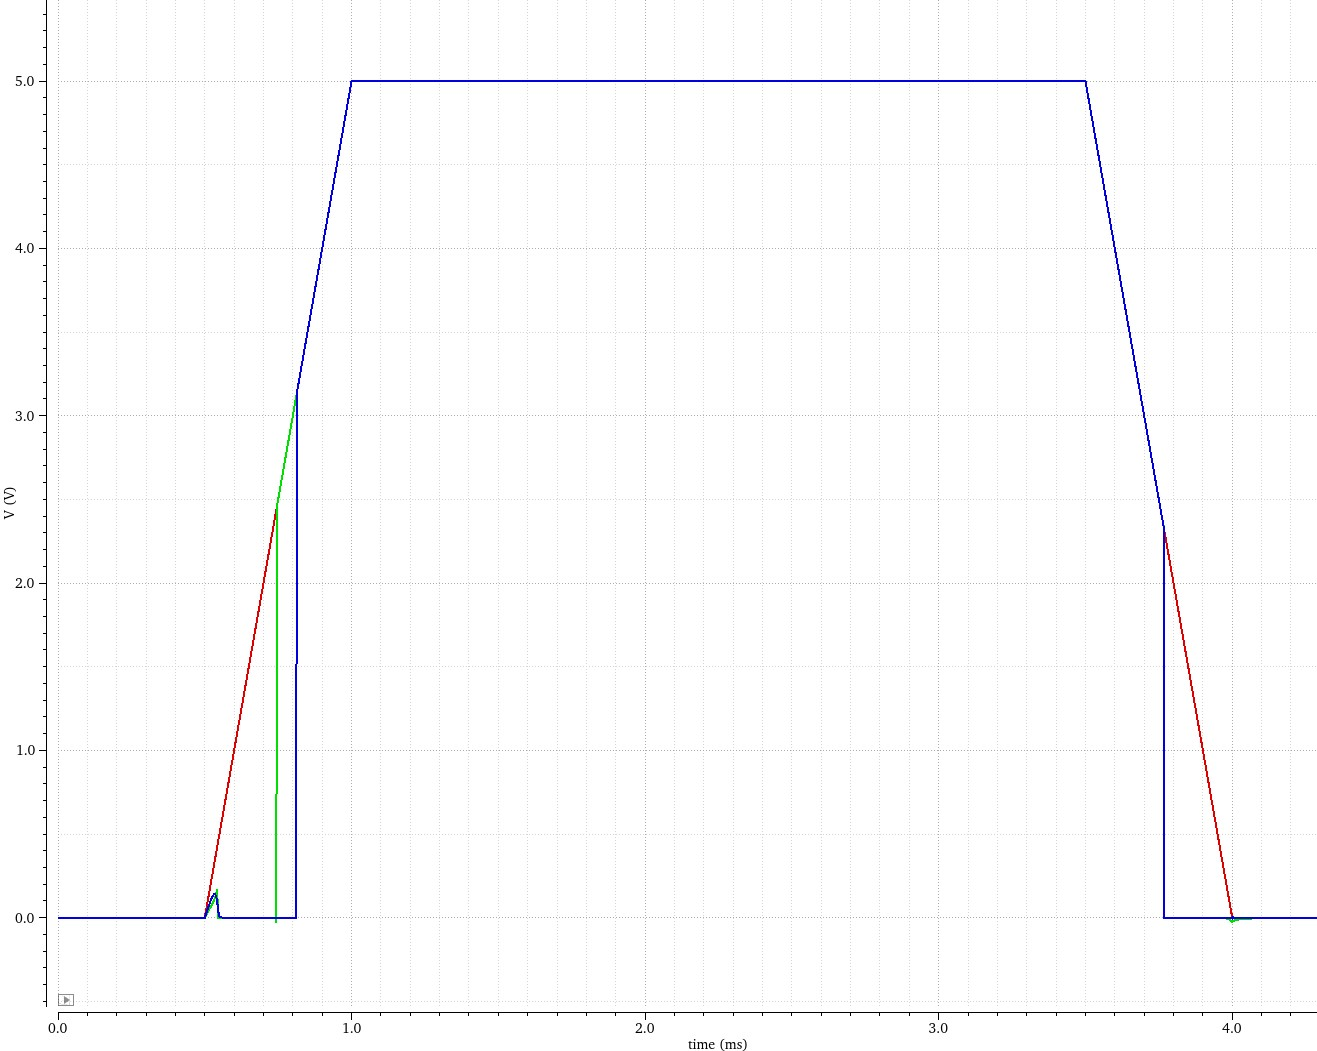
\includegraphics[width=0.8\textwidth]{figures/CD/waveform_standard.jpg}};

        % Legende hinzufügen
        \begin{scope}[shift={(0,-1)}]  % Position der Legende anpassen
            \draw[white] (0,0) rectangle (3.2,1.8); % Hintergrund für die Legende
            \node[anchor=west] at (-2,0.5) {\footnotesize\textcolor{red}{\textbf{---}} Betriebsspannung ($V_{DD}$)};
            \node[anchor=west] at (2,0.5) {\footnotesize\textcolor{green}{\textbf{---}} Komparatorausgang ($V_{comp}$)};
            \node[anchor=west] at (6.5,0.5) {\footnotesize\textcolor{blue}{\textbf{---}} Ausgang PoR-Schaltung ($V_{out}$)};
        \end{scope}
    \end{tikzpicture}
    \caption[Spannungsverläufe der Power-on-Reset-Schaltung]{: Spannungsverläufe der Power-on-Reset-Schaltung}
    \label{fig:por_waveform}
\end{figure}
 sodass beide Varianten nun so weiter optimiert werden können, um exakt den vorgegebenen Spezifikationen zu entsprechen. Dies umfasst unter anderem die präzise Abstimmung der Schaltschwellen sowie die Sicherstellung, dass die Reset-Signale unter allen Betriebsbedingungen rechtzeitig und zuverlässig zur Verfügung stehen. So wird sichergestellt, dass die \gls{por}-Schaltung sowohl im analogen als auch im digitalen Bereich ihre Aufgabe erfüllt und sich keine undefinierten Zustände im System einstellen. 
\chapter{Verifizierung}\label{chap:Verifizierung}
Die Einhaltung der in Polarion\footnote{\url{https://plm.sw.siemens.com/de-DE/polarion/} --\,zuletzt am 21.~Februar~2025 erfolgreich aufgerufen.} dokumentierten Spezifikationen ist ein zentraler Bestandteil der Entwicklung der \gls{por}-Schaltung. Diese Spezifikationen definieren die funktionskritischen Parameter der Schaltung, wie beispielsweise die Einschaltverzögerung, die Reset-Aktivierungsschwelle und die Reaktionszeit bei Spannungsabfall. Da der \gls{por} eine essenzielle Rolle für das fehlerfreie Hochfahren und Zurücksetzen des gesamten Systems spielt, müssen diese Parameter innerhalb der definierten Grenzen liegen, um eine zuverlässige Initialisierung des Chips sicherzustellen.

\section{Spezifikationen}
Nachdem die grundlegende Funktionsweise der einzelnen Funktionsblöcke erfolgreich simuliert und validiert wurde, erfolgte eine gezielte Anpassung der Bauelemente, um die spezifizierten Anforderungen zu erfüllen. Die Schaltung wurde mit der Cadence\footnote{\url{https://www.cadence.com/en_US/home.html}  --\,zuletzt am 21.~Februar~2025 erfolgreich aufgerufen.}-Virtuoso-Design-Suite entworfen und getestet. Der Fokus lag dabei auf der korrekten Implementierung der verzögerten Aktivierung sowie der schnellen Reaktion des Reset-Signals beim Abschalten der Versorgungsspannung und dem Einstellen der Schwell- und Reset-Spannung des Komparators. 

Zunächst erfolgte die Simulation unter nominalen Bedingungen, um sicherzustellen, dass die Funktionsblöcke sich in Kombination wie zu erwarten verhalten. Zu Beginn wurden die Schaltschwellen des Komparators mit Hilfe der Widerstände eingestellt, um sichergehen zu können, dass sich die Reset-Spannung ($V_L$ siehe \autoref{fig:Reset-Spannung}) unter Schwellspannung ($V_H$ siehe \autoref{fig:Schwellspannung})befindet. Anschließend wurde besonders die Lade- und Entladezeit des Kondensators für die Reset-Freigabe analysiert, damit sich im System keine undefinierten Zustände einstellen, wenn es zu Spannungsschwankungen kommt. Durch Anpassungen und eine erneute Simulation konnte die Grundfunktionalität der \gls{por}-Schaltung verifiziert werden. Um die vorgegeben Spezifikationen bestmöglich zu erreichen, wurden gezielte Anpassungen an der Dimensionierung der Transistoren vorgenommen. Nachdem sich die Werte der Schaltung in dem Bereich der Spezifikationen befanden, wurde die nominale Corner-Simulation bei 27$^{\circ}$C, um verschiedene Prozesstypen sowie die maximalen Temperaturen erweitert. 

\section{Corner-Simulation}
Die Entwicklung einer robusten \gls{por}-Schaltung erfordert eine detaillierte Analyse der Schaltungsperformance unter verschiedenen Betriebsbedingungen. In modernen Halbleiterprozessen unterliegen Transistoren und passive Bauelemente\footnote{Dazu zählen u.a. Widerstände und Kondensatoren} signifikanten Variationen, die durch Unterschiede in der Produktion, Umgebungstemperatur und Versorgungsspannung verursacht werden. Um die korrekte Funktion der Schaltung sicherzustellen, wurde zuerst eine Corner-Simulation durchgeführt. Diese Simulation ermöglicht es, die Auswirkungen von \gls{pvt} systematisch zu untersuchen und gegebenenfalls gezielte Entwurfsanpassungen vorzunehmen. Werden Prozess- und Temperaturvariationen unzureichend berücksichtigt, kann dies dazu führen, dass die \gls{por}-Schaltung unter bestimmten Bedingungen fehlerhaft arbeitet. Beispielsweise könnte die Schaltung in einem \enquote{schnellen} Prozess-Corner~(höhere Elektronenmobilität, geringer Widerstände) zu früh oder in einem \enquote{langsamen} Prozess-Corner~(geringere Mobilität, höhere Widerstände) zu spät auslösen. Beides könnte schwerwiegende Konsequenzen für das Gesamtsystem haben, da Teile der restlichen Schaltung möglicherweise in einem undefinierten Zustand starten. In der Cadence-Virtuoso-ADE-Explorer-Umgebung werden daher verschiede Prozessvariationen und Temperaturbedingungen systematisch getestet. Die Standard-Prozesscorners in modernen CMOS-Technologien lassen sich wie folgt klassifizieren: 
\begin{table}[h!]
    \centering
    \footnotesize
    \begin{tabular}{c|c|c|c|c}
        \textbf{\makecell{Abkürzung}} &
        \textbf{\makecell{Bedeutung}} &
        \textbf{\makecell{Verhalten\\ NMOS}} &
        \textbf{\makecell{Verhalten\\ PMOS}} &
        \textbf{\makecell{Verhalten passive\\ Bauelemente}} \\
        \midrule
        ttt & typical-typical-typical & Nominal & Nominal & Nominal \\
        sss & slow-slow-slow & Langsam & Langsam & Langsam \\
        fff & fast-fast-fast & Schnell & Schnell & Schnell \\
        sft & slow-fast-typical & Langsam & Schnell & Nominal \\
        fst & fast-slow-typical & Schnell & Langsam & Nominal \\
        sfs & slow-fast-slow & Langsam & Schnell & Langsam \\
        sff & slow-fast-fast & Langsam & Schnell & Schnell \\
        fss & fast-slow-slow & Schnell & Langsam & Langsam \\
        fsf & fast-slow-fast & Schnell & Langsam & Schnell \\
    \end{tabular}
    \caption{Transistor- und Bauelement-Konfigurationen der Corner-Simulation}
    \label{tab:transistor_configurations}
\end{table}

Bei dieser Simulation können verschiedene Probleme auftreten, die eine Anpassung des Entwurfs erforderlich machen. Die Schwellspannung von \gls{nmos}- und \gls{pmos}-Transistoren kann sich je nach Prozess-Corner erheblich unterscheiden. In langsamen Corners (sss) ist die Schwellspannung typischerweise höher, wodurch sich die Transistoren langsamer schalten. In schnellen Corners (fff) wird diese reduziert, sodass die Transistoren früher schalten. Dadurch verschiebt sich die Reset-Schwelle der \gls{por}-Schaltung, was eine fehlerhafte oder verzögerte Initialisierung des Systems zur Folge haben kann. Die Kapazität des Kondensators~$C$ kann aufgrund von Fertigungstoleranzen schwanken. In einem sss-Prozess kann die Kapazität größer sein als erwartet, was die Ladezeit verlängert. In einem fff-Prozess ist die Kapazität möglicherweise geringer, sodass die Reset-Verzögerung verkürzt wird. 

Ohmsche Widerstände und Kapazitäten sind stark temperaturabhängig. Bei niedrigen Temperaturen von -40$^{\circ}C$ kann der Widerstand ansteigen, wodurch eine Verzögerung in der Schaltung entstehen kann. Hohe Temperaturen während des Betriebs können zu erhöhten Leckströmen und einer ungewollten Entladung des Kondensators führen, wodurch das Reset zu früh freigegeben wird. Während Prozessen wie sft (slow-fast-typical) oder fst (fast-slow-typical) arbeiten \gls{nmos}- und \gls{pmos}-Transistoren mit unterschiedlicher Geschwindigkeit. Dies kann zu asymmetrischem Verhalten im Schaltungsentwurf führen. Bei \gls{por}-Schaltungen muss das Reset-Signal sauber und zuverlässig detektiert werden, weshalb auch diese Simulation kritisch betrachtet werden muss.

Die Simulationsergebnisse (siehe \autoref{tab:corner_old_summary}) zeigen, dass die \gls{por}-Schaltung nur für wenige Corner-Fälle den vorgegebenen Spezifikationen entspricht, was auch durch Anpassungen der Kanalbreite und Länge der einzelnen Transistoren nicht stabilisiert werden kann. Grund dafür ist, dass Ohmsche Widerstände in integrierten Schaltungen signifikanten Fertigungsstreuungen aufgrund von Schwankungen in der Dicke und Dotierung des Halbleitermaterials unterliegen. Aber vor allem der Widerstandswert ändert sich mit der Temperatur, da der \gls{tcr} von Wiederständen relativ hoch ist \cite{ADofIntegratedCircuits}. Dadurch sind die Schwankungen der Referenzspannung (siehe \autoref{fig:Vref_fluctuation_old}) mit $\approx$ 320mV zu groß, um die Schaltung über die Corner-Simulation den Spezifikationen anzupassen. Deswegen muss der Entwurf für die bestehende Generierung der Referenzspannung aus \autoref{fig:Vref_old} überarbeitet werden.    
{\begin{table}[H]
    \centering
    \small
    \begin{tabular}{c|l|c|c|c}
        {\rotatebox{90}{\parbox{1.8cm}{\textbf{Spannung}}}} &
        \textbf{\makecell{Werte}} &
        \textbf{\makecell{Spezifikation}} &
        \textbf{\makecell{Min. Wert}} &
        \textbf{\makecell{Max. Wert}} \\
        \midrule

        \multirow{5}{*}{\rotatebox{90}{5 V}} &
        Verzögerung steigende Flanke & 20 us $\leq$ x $\leq$ 130 us & 20.27 us & 117.9 us \\
        & Verzögerung fallende Flanke & $\leq$ 1 us & 37.99 ns & 123.8 ns \\
        & Schwellspannung steigend & 2.2 V $\leq$ x $\leq$ 2.6 V & \cellcolor{lightred}1.811 V & \cellcolor{lightred}2.946 V \\
        & Schwellspannung fallend & 2.1 V $\leq$ x $\leq$ 2.5 V & \cellcolor{lightred}1.743 V & \cellcolor{lightred}2.849 V \\
        & Hysterese & 50 mV $\leq$ x $\leq$ 120 mV & 67.85 mV & 98.69 mV \\
        \midrule
    \end{tabular}
    \caption{Ergebnisse Corner-Simulation Widerstands-basierte PoR-Schaltung}
    \label{tab:corner_old_summary}
\end{table}

\subsection{Anpassung Referenzspannung}
Im Gegensatz dazu bietet die auf Transistoren basierende Referenzspannung (siehe \autoref{fig:Vref&Vres}) eine bessere Kompensation gegenüber Prozess- und Temperaturabweichungen. MOS-Tran\-sistoren in speziellen Konfigurationen, beispielsweise in Spannungsteiler- oder Stromspiegelstrukturen, können die Referenzspannung deutlich stabilisieren, da sie durch einen gezielten Schaltungsentwurf eine geringere Sensitivität gegenüber Fertigungsstreuungen aufweisen \cite{DesignOfAnalogCMOSIntegratedCircuits}.
In dem neuen Entwurf wird das Gate des nativen NMOS-Transistors $N_1$ durch die Spannung $V_{gate}$ gesteuert. $V_{gate}$ wiederum wird durch den Spannungsteiler aus $R_0$ und $N_0$ generiert. $N_1$ und $N_2$ bilden eine spannungsgesteuerte Referenzquelle, die durch die Spannung von $V_{gate}$ auch über Prozess- und Temperaturschwankungen konstanter ist. Damit der Komparator eine stabile Referenzspannung für die Spannungsversorgung hat, wurde der Entwurf für die Generierung der Referenzspannung (siehe \autoref{fig:Vref&Vres}) angepasst.  
%\vspace{1.5\baselineskip}
\begin{figure}[H]
    \begin{center}
        \begin{circuitikz}[european]
            \ctikzset{tripoles/mos style/arrows}[line width=thick, european]
            % Widerstand
            \draw (-4,4) coordinate(resistor-begin) to[resistor, l={$R_0$}] (-4,1) coordinate(resistor-end);
                %(-5.5,3) -- (-4.5,3) node[above, midway]{$Vdd$};
            
            % NMOS Transistor
            \draw (-4,-0.5) node[nmos, anchor=drain] (nmosL) {$N_0$};

            % NMOS Transistoren R 
            \draw (-1.5,3.25) node[nmosd, anchor=drain] (nmosL1) {$N_1$}
                %(nmosL1.gate) -- ++(-0.5,0) |- (resistor-end);
                (resistor-end) -- ++(1,0) |- (nmosL1.gate);
            \draw (-1.5,-1) node[nmos, anchor=drain] (nmosL2) {$N_2$}
                (nmosL1.source) -- (nmosL2.drain) coordinate [pos=0.5](nmosMP) % Verbindung & Mittelpunkt zwischen nmos
                (nmosMP) node[circle, fill, inner sep=1.5pt]{}
                (nmosL2.gate) -- ++(-0.25,0) |- (nmosMP)
                node[above, xshift=-20pt]{$V_{ref}$};
                
            
            % Verbindung von Drain des NMOS mit Widerstand
            \draw (resistor-end) -- (nmosL.drain);
            \draw (nmosL.gate) -- ++(-0.25,0) |- (resistor-end)
                node[circle, fill, inner sep=1.5pt]{}
                node[above, midway]{$V_{gate}$};
            %
            %*************************************************************************
            %
            % Widerstand R
            \draw (0,4.5) coordinate (resistor-begin1) to[resistor, l={$R_1$}] (0,2) coordinate (resistor-end1);
            \draw (0,2) coordinate (resistor-begin2) to[resistor, l={$R_2$}] (0,-1) coordinate (resistor-end2);
            \draw (0,-1) coordinate (resistor-begin3) to[resistor, l={$R_3$}] (0,-3.5) coordinate (resistor-end3);

            % NMOSR 
            \draw (3,2) node[nmos, rotate=270] (nmosR1) {}
                node at (nmosR1.center) [anchor=center, yshift=-10pt] {$N_3$}
                (nmosR1.source) -- (resistor-end1) % Verbinung zu Wiederständen 
                node[circle, fill, inner sep=1.5pt]{}; % Punkt am Ende der Verbindung 
            \draw (3,-1) node[nmos, rotate=270] (nmosR2) {}
                node at (nmosR2.center) [anchor=center, yshift=-10pt] {$N_4$}
                (nmosR2.source) -- (resistor-end2)
                node[circle, fill, inner sep=1.5pt]{};

            % NMOS Drain Verbindung
            \draw (nmosR1.drain) -- ++ (0.25,0) % horizontal nach rechts
                -- ++ (0,-3) coordinate (comp) % vertikale Linie 
                node[circle, fill, inner sep=1.5pt]{};

            \draw (nmosR1.gate) -- ++(0,0.25) -- ++(-0.75,0) 
                node[above, midway]{$V_{res}$};
            \draw (nmosR2.gate) -- ++(0,0.25) -- ++(-0.75,0)
                node[above, midway]{$V_{res0}$};

            % Dreieck am Ende von Vcomp
            \draw (6.75,-0.51) node[op amp] (triangle){}
                (triangle.+) -- (nmosR2.drain);
            \draw (triangle) node[above, yshift=27pt] {Komparator};  

            \draw (triangle.-) -- ++(-0.5,0) node[above]{$V_{ref}$};

            % Verbindung Ground
            \draw (nmosL.source) |- (resistor-end3)
                (nmosL2.source) |- (resistor-end3) coordinate[pos=0.5](gndM)
                (gndM) -- ++(0,-0.25) node[sground]{}
                    node[right, xshift=5pt, yshift=-5pt]{Gnd}
                (gndM) node[circle, fill, inner sep=1.5pt]{}; 

            % Verbindung VDD
            \draw (resistor-begin) |- (resistor-begin1)
                (nmosL1.drain) |- (resistor-begin1) coordinate[pos=0.5](vddM)
                (vddM) node[circle, fill, inner sep=1.5pt]{}
                (vddM) -- ++(0,0.5) coordinate(vddA)
                (vddA) -- ++(-0.5,0)
                (vddA) -- ++(0.5,0)
                (vddA) node[above] {$V_{DD}$};

        \end{circuitikz}
    \end{center}
    \caption[Generierung des Referenzstrom durch Transistor]{\\Quelle: Generierung des Referenzstrom durch Transistor (Eigene Darstellung)}
    \label{fig:Vref&Vres}
\end{figure}
%\vspace{1.5\baselineskip}
Bei dem \gls{nmos}-Transistor $N_1$ handelt es sich um einen Native Transistor, da es sonst zu einer Verzögerung in der Generierung der Referenzspannung kommt und der Schaltvorgang des Komparator nicht richtig ausgeführt werden kann. Der Transistor $N_2$ fungiert als \gls{nmos}-Diode. Die so entstehende Referenzspannung $V_{ref}$ hängt von der Wahl des Widerstands $R_0$ sowie von den transistorabhängigen Parametern wie der Threshold-Spannung ($V_{th}$) und dem Stromverstärkungsfaktor ab. Die Schaltung stellt sicher, dass $V_{ref}$ über einen weiten Bereich stabil bleibt und unabhängig von Versorgungsspannungsschwankungen oder externen Störungen eine konstante Referenz bildet \cite{CircuitDesigLayoutAndSimulation}. Durch diese Entwurfsanpassung konnte die Schwankung der Referenzspannung um ca. $^1/_3$ auf $\approx$ 99 mV wie in \autoref{fig:Vref_Variation} zu sehen ist, verringert werden. Dies führt dazu, dass die Schaltung auch über die Corner-Simualation den Spezifikationen entspricht. \autoref{tab:corner_summary1.5} zeigt die wichtigsten Analysewerte der Simulation für die \gls{por}-Schaltung des digitalen Teils: 
\begin{table}[H]
    \centering
    \small
    \begin{tabular}{c|l|c|c|c}
        {\rotatebox{90}{\parbox{1.8cm}{\textbf{Spannung}}}} &
        \textbf{\makecell{Werte}} &
        \textbf{\makecell{Spezifikation}} &
        \textbf{\makecell{Min. Wert}} &
        \textbf{\makecell{Max. Wert}} \\
        \midrule

        \multirow{5}{*}{\rotatebox{90}{5 V}} &
        Verzögerung steigende Flanke & 20 us $\leq$ x $\leq$ 155 us & 20.78 us & 153.9 us \\
        & Verzögerung fallende Flanke & $\leq$ 1 us & 48.99 ns & 206.3 ns \\
        & Schwellspannung steigend & 1.1 V $\leq$ x $\leq$ 1.45 V & 1.133 V & 1.443 V \\
        & Schwellspannung fallend & 1.05 V $\leq$ x $\leq$ 1.4 V & 1.066 V & 1.359 V \\
        & Hysterese & 50 mV $\leq$ x $\leq$ 90 mV & 66.97 mV & 84.79 mV \\
        \midrule
    \end{tabular}
    \caption{Ergebnisse Corner-Simulation PoR-Schaltung für den digitalen Teil}
    \label{tab:corner_summary1.5}
\end{table}





































Die Analysewerte der Corner-Simulation der \gls{por}-Schaltung für den analogen Schaltungsteil werden in \autoref{tab:corner_summary} dargestellt. Dabei überschreitet der Maximalwert für den fallenden Schwellenwert mit 15 mV und befindet sich damit außerhalb der Spezifikation. Da es sich bei der Corner-Simulation um ein Worst-Case-Szenario handelt, ist bei dieser geringen Abweichung keine weitere Anpassung notwendig.
\begin{table}[H]
    \centering
    \small
    \begin{tabular}{c|l|c|c|c}
        {\rotatebox{90}{\parbox{1.8cm}{\textbf{Spannung}}}} &
        \textbf{\makecell{Werte}} &
        \textbf{\makecell{Spezifikation}} &
        \textbf{\makecell{Min. Wert}} &
        \textbf{\makecell{Max. Wert}} \\
        \midrule

        \multirow{5}{*}{\rotatebox{90}{5 V}} &
        Verzögerung steigende Flanke & 20 us $\leq$ x $\leq$ 130 us & 24.37 us & 126.5 us \\
        & Verzögerung fallende Flanke & $\leq$ 1 us & 34.53 ns & 138 ns \\
        & Schwellspannung steigend & 2.2 V $\leq$ x $\leq$ 2.6 V & 2.206 V & 2.577 V \\
        & Schwellspannung fallend & 2.1 V $\leq$ x $\leq$ 2.5 V & 2.153 V & \cellcolor{lightyellow}2.515 V \\
        & Hysterese & 50 mV $\leq$ x $\leq$ 120 mV & 52.96 mV & 63.08 mV \\
        \midrule
    \end{tabular}
    \caption{Ergebnisse Corner-Simulation PoR-Schaltung für den analogen Teil}
    \label{tab:corner_summary}
\end{table}

\section{Monte-Carlo-Simulation}
Nachdem die \gls{por}-Schaltung die Spezifikationen in der Corner Simulation erfüllt, wurde abschließend eine \gls{mc}-Simulation durchgeführt. Diese Simulation testet die Zuverlässigkeit der Schaltung unter realen Fertigungsbedingungen. Während die Corner-Simulation systematische Schwankungen (Worst-Case-Szenarien) untersucht, ermöglicht die \gls{mc}-Simulation eine statistische Analyse zufälliger Variationen, die während der Herstellung auftreten können. In Cadence können \gls{mc}-Simulationen in drei verschiedene Kategorien unterteilt werden, welche in diesem Fall mit jeweils 200 Iterationen ausgeführt wurden. Das bedeutet, für jeden Durchlauf wurden den Bauteilen zufällige Parameter (in Form einer Gaußverteilung), die durch die Fertigung auftreten können, zugeteilt und berechnet. 

Bei der Process-Simulation innerhalb der \gls{mc}-Simulation werden alle Transistoren und Bauteile mit zufälligen Abweichungen versehen, welche globale Fertigungsschwankungen widerspiegeln. Diese Schwankungen wirken sich auf alle Bauteile einer Wafer-Charge\footnote{\url{https://heinen-elektronik.de/glossar/wafer/} --\,zuletzt am 27.~Februar~2025 erfolgreich aufgerufen.} gleichermaßen aus. 

Die Mismatch-Simulation untersucht lokale Unterschiede zwischen identischen Bauelementen. Dazu zählen beispielsweise kleine Abweichungen zwischen den Transistoren, die einen Differenzverstärker bilden. Das Ergebnis ist eine Verteilung der Offset-Spannung oder Stromabweichung aufgrund von Fertigungsunterschieden zwischen benachbarten Bauelementen.

Die All-Simulation ist eine Kombination aus lokalen Mismatch-Variationen und globalen Prozessabweichungen, um ein realitätsnahes Verhalten der Schaltung zu simulieren. Sie stellt sicher, dass weder großflächige noch feinere Variationen in der Fertigung sich außerhalb der spezifizierten Grenzen befinden. 

\subsection{Einfluss von Flankenzeiten auf die Funktionalität}
Die drei Varianten der \gls{mc}-Simulation werden unter Variation der Anstiegs- und Abfallzeiten (Flanken) der Versorgungsspannung ausgeführt. Die Anstiegszeit beschreibt die Zeit, welche die Versorgungsspannung benötigt, um von 0~V auf 1.5~V (für den digital Teil) oder 5~V~(für den analogen Teil) anzusteigen. Bei der Abfallzeit handelt es sich dementsprechend um die Dauer des Abfallen der Versorgungsspannung beim Ausschalten des Systems. Diese Parameter sind besonders für \gls{por}-Schaltungen von großer Bedeutung, da sie direkt beeinflussen, wann die interne Referenzspannung aufgebaut wird und wie schnell der Komparator in den aktiven Zustand übergeht. 

Bei kurzen Anstiegszeiten (z.B. 10 ms) steigt die Versorgungsspannung sehr schnell an, wodurch sich die Schaltung innerhalb kürzester Zeit initialisieren muss. Dies stellt erhöhte Anforderungen an die Generierung der Referenzspannung und an die Stabilität des Komparators bei schnell wechselnden Flanken. Besonders kritisch ist dabei die zuverlässige Erkennung des Spannungsniveaus sowie die saubere Generierung des Reset-Signals, bevor nachfolgende Schaltungsteile aktiviert werden. Längere Anstiegszeiten (z.B. 100 ms) führen hingegen zu einem langsameren Spannungsanstieg. Dabei hat die Schaltung mehr Zeit, die interne Referenzspannung aufzubauen und die Eingangsbedingungen des Komparators zu stabilisieren. Allerdings können bei sehr langsamen Anstiegszeiten unerwünschte Zwischenzustände auftreten, bei denen die Spannung bereits hoch genug ist, um Teilschaltungen zu aktivieren, während die Reset-Bedingungen noch nicht sicher erfüllt sind. Dies kann insbesondere in Kombination mit Prozess- und Mismatch-Schwankungen zu einer erhöhten Fehleranfälligkeit führen.

Ähnliche Effekte treten bei der Variation der fallenden Flanke auf. Ein schnelles Abschalten~(10 ms) entlädt die Versorgung sehr abrupt, was dazu führen kann, dass das Reset-Signal nicht rechtzeitig ausgelöst wird. Bei einem langsamen Spannungsabfall (100 ms) können unerwünschten Restströmen oder Fehlinterpretationen von Schaltzuständen auftreten. Damit sich keine falschen Zustände im System einstellen, muss das Reset-Signal sowohl für langsame als auch schnell fallende Flanken zuverlässig ausgelöst werden. 

\subsection{Analyse der Abweichungen in der Monte-Carlo-Simulation}
Die \gls{mc}-Process-Simulation zeigte, dass die Schwellwerte der steigenden und fallenden Flanken fast 200 mV außerhalb der spezifizierten Grenzen liegen wie in \autoref{tab:MCProcess100} zu sehen ist. Dieses Verhalten ist insofern ungewöhnlich, da die Corner-Simulationen, die die Worst-Case-Bedingungen abdecken sollen. Die in der Spezifikation angegeben Werte werden an den geprüften Temperaturpunkten (-40 $^{\circ}$C, 27 $^{\circ}$C und 125 $^{\circ}$C) sicher einhalten. Dass die \gls{mc}-Process-Simulation bei nominaler Temperatur von 27 $^{\circ}$C eine so deutliche Abweichung aufweist, deutet auf eine Unstimmigkeit im Simulations- oder Modellierungsprozess hin. Aus diesem Grund muss die Dokumentation der Cadence-Simulation noch einmal genauer überprüft, um die Ursache dieser Abweichung herauszufinden. Bisherige Tests deuten darauf hin, dass der Fehler durch den nativ Transistor verursacht wird, auch wenn die Wert der \gls{por}-Schaltung für den digitalen Teil den Spezifikationen entsprechen. 
\begin{table}[H]
    \centering
    \small
    \begin{tabular}{c|l|c|c|c}
        {\rotatebox{90}{\parbox{1.8cm}{\textbf{Spannung}}}} &
        \textbf{\makecell{Werte}} &
        \textbf{\makecell{Spezifikation}} &
        \textbf{\makecell{Min. Wert}} &
        \textbf{\makecell{Max. Wert}} \\
        \midrule

        \multirow{5}{*}{\rotatebox{90}{5 V}} &
        Verzögerung steigende Flanke & 20 us $\leq$ x $\leq$ 130 us & 46.25 us & 89.11 us \\
        & Verzögerung fallende Flanke & x $\leq$ 1 us & 57.65 ns & 79.79 ns \\
        & Schwellspannung steigend & 2.2 V $\leq$ x $\leq$ 2.6 V & \cellcolor{lightred}2.088 V & \cellcolor{lightred}2.722 V \\
        & Schwellspannung fallend & 2.1 V $\leq$ x $\leq$ 2.5 V & \cellcolor{lightred}2.038 V & \cellcolor{lightred}2.659 V \\
        & Hysterese & 50 mV $\leq$ x $\leq$ 120 mV & \cellcolor{lightyellow}49.92 mV & 62.88 mV \\
        \midrule

        \multirow{5}{*}{\rotatebox{90}{1.5 V}} &
        Verzögerung steigende Flanke & 20 us $\leq$ x $\leq$ 230 us & 42.36 us & 77.56 us \\
        & Verzögerung fallende Flanke & x $\leq$ 1 us & 80.05 ns & 118.6 ns \\
        & Schwellspannung steigend & 1.1 V $\leq$ x $\leq$ 1.45 V & 1.147 V & 1.445 V \\
        & Schwellspannung fallend & 1.05 V $\leq$ x $\leq$ 1.4 V & 1.079 V & 1.361 V \\
        & Hysterese & 50 mV $\leq$ x $\leq$ 120 mV & 68.14 mV & 84.18 mV \\
        \midrule
        
    \end{tabular}
    \caption{MC-Process-Simulation mit Anstiegs-und Abfallzeit von 100~ms}
    \label{tab:MCProcess100}
\end{table}

Bei den in \autoref{tab:MCMismatch100} zu sehenden Ergebnissen der \gls{mc}-Mismatch-Simulation liegen die Schwellwerte der Flanken und die anderen entschiedenen Messwerte innerhalb der Spezifikation. Auch die Schwankungsbreite der Ergebnisse ist bei der Mismatch-Simulation geringer als bei der Corner-Simulation, was grundsätzlich dem erwarteten Verhalten entspricht. Diese Beobachtung gilt sowohl für die \gls{por}-Schaltung im analogen (5~V) als auch im digitalen (1,5~V) Schaltungsteil.
\begin{table}[H]
    \centering
    \small
    \begin{tabular}{c|l|c|c|c}
        {\rotatebox{90}{\parbox{1.8cm}{\textbf{Spannung}}}} &
        \textbf{\makecell{Werte}} &
        \textbf{\makecell{Spezifikation}} &
        \textbf{\makecell{Min. Wert}} &
        \textbf{\makecell{Max. Wert}} \\
        \midrule
        
        \multirow{5}{*}{\rotatebox{90}{5 V}} &
        Verzögerung steigende Flanke & 20 us $\leq$ x $\leq$ 130 us & 40.02 us & 108.9 us \\
        & Verzögerung fallende Flanke & x $\leq$ 1 us & 63.88 ns & 72.03 ns \\
        & Schwellspannung steigend & 2.2 V $\leq$ x $\leq$ 2.6 V & 2.35 V & 2.457 V \\
        & Schwellspannung fallend & 2.1 V $\leq$ x $\leq$ 2.5 V & 2.293 V & 2.4 V \\
        & Hysterese & 50 mV $\leq$ x $\leq$ 120 mV & 45.44 mV & 57.49 mV \\
        \midrule

        \multirow{5}{*}{\rotatebox{90}{1.5 V}} &
        Verzögerung steigende Flanke & 20 us $\leq$ x $\leq$ 230 us & 33.84 us & 77.86 us \\
        & Verzögerung fallende Flanke & x $\leq$ 1 us & 84.6 ns & 108 ns \\
        & Schwellspannung steigend & 1.1 V $\leq$ x $\leq$ 1.45 V & 1.219 V & 1.343 V \\
        & Schwellspannung fallend & 1.05 V $\leq$ x $\leq$ 1.4 V & 1.146 V & 1.265 V \\
        & Hysterese & 50 mV $\leq$ x $\leq$ 120 mV & 72.77 mV & 78.94 mV \\
        \midrule
        
    \end{tabular}
    \caption{MC-Mismatch-Simulation mit Anstiegs-und Abfallzeit von 100~ms}
    \label{tab:MCMismatch100}
\end{table}

Da die \gls{mc}-All-Simulation eine Kombination aus Process- und Mismatch-Variatio\-nen ist, treten die beschriebenen Abweichungen auch bei dieser Simulation auf (siehe \autoref{tab:MCAll100}). Die Schwellwerte der Flanken liegen dabei ebenfalls außerhalb der spezifizierten Grenzen. Bei dieser Simulation sind auch die Wert der \gls{por}-Schaltung bei einer Betriebsspannung von 1.5~V außerhalb der Werte der Corner-Simulation. 
\begin{table}[H]
    \centering
    \small
    \begin{tabular}{c|l|c|c|c}
        {\rotatebox{90}{\parbox{1.8cm}{\textbf{Spannung}}}} &
        \textbf{\makecell{Werte}} &
        \textbf{\makecell{Spezifikation}} &
        \textbf{\makecell{Min. Wert}} &
        \textbf{\makecell{Max. Wert}} \\
        \midrule

        \multirow{5}{*}{\rotatebox{90}{5 V}} &
        Verzögerung steigende Flanke & 20 us $\leq$ x $\leq$ 130 us & 38.94 us & 115.5 us \\
        & Verzögerung fallende Flanke & x $\leq$ 1 us & 57.15 ns & 81.63 ns \\
        & Schwellspannung steigend & 2.2 V $\leq$ x $\leq$ 2.6 V & \cellcolor{lightred}2.058 V & \cellcolor{lightred}2.75 V \\
        & Schwellspannung fallend & 2.1 V $\leq$ x $\leq$ 2.5 V & \cellcolor{lightred}2.008 V & \cellcolor{lightred}2.686 V \\
        & Hysterese & 50 mV $\leq$ x $\leq$ 120 mV & \cellcolor{lightyellow}49.47 mV & 64.14 mV \\
        \midrule

        \multirow{5}{*}{\rotatebox{90}{1.5 V}} &
        Verzögerung steigende Flanke & 20 us $\leq$ x $\leq$ 230 us & 36.93 us & 88.91 us \\
        & Verzögerung fallende Flanke & x $\leq$ 1 us & 77.38 ns & 129.2 ns \\
        & Schwellspannung steigend & 1.1 V $\leq$ x $\leq$ 1.45 V & 1.123 V & \cellcolor{lightyellow}1.452 V \\
        & Schwellspannung fallend & 1.05 V $\leq$ x $\leq$ 1.4 V & 1.055 V & 1.368 V \\
        & Hysterese & 50 mV $\leq$ x $\leq$ 120 mV & 67.06 mV & 83.75 mV \\
        \midrule
        
    \end{tabular}
    \caption{MC-All-Simulation mit Anstiegs-und Abfallzeit von 100~ms}
    \label{tab:MCAll100}
\end{table}

Weitere Analysen konzentrieren sich daher speziell auf die Modellparameter des nativen Transistors sowie die genaue Prozessbeschreibung innerhalb der Cadence-Umgebung, um die Abweichung einzugrenzen und gegebenenfalls Korrekturmaßnahmen einzuleiten oder den Entwurf noch mal anzupassen. 

Die Ergebnisse der \gls{mc}-Simulationen bei Anstiegs-und Abfallzeiten von 10~ms~(siehe~\ref{tab:MCProcess10}, \ref{tab:MCMismatch10}, \ref{tab:MCAll10}) liegen unterscheiden sich nur gering von den Ergebnissen der Simulationen bei 100~ms. In beiden Fällen bewegen sich die Werte, abgesehen von den bekannten Abweichungen durch den Nativ Transistor, innerhalb der spezifizierten Grenzen.  

Um sicherstellen zu können, dass das Reset-Signal auch bei schnellem Flankenwechsel zuverlässig funktioniert, wurde noch eine \gls{mc}-All-Simulation mit einer Anstiegs-und Abstiegszeit von nur 1~ms durchgeführt. Wie zuvor liegen auch bei dieser Simulation die Werte der Schwellspannung außerhalb der Spezifikation, dennoch bleibt die Grundlegende Funktion der Schaltung erhalten. Die Verzögerung und Freigabe des Reset-Signals findet innerhalb der spezifizierten Grenzen statt (siehe \ref{tab:MCAll1}), wodurch eine zuverlässige Funktion der \gls{por}-Schaltungen bestätigt werden konnte. 
\chapter{Fazit}\label{chap:Schluss}
Im Rahmen dieser Arbeit wurde eine \glsentrylong{por}-Schaltung für einen neu entwickelten Chip entworfen, der sowohl analoge als auch digitale Funktionsblöcke enthält. Aufgrund der unterschiedlichen Anforderungen dieser beiden Bereiche wurden separate \gls{por}-Schaltungen entwickelt und gezielt an die jeweiligen Versorgungsspannungen angepasst. Der Fokus lag dabei auf der Verzögerung und einer sofortigen Freigabe des Reset-Signals. Die ursprüngliche widerstandsbasierte Referenzspannung erwies sich in der Corner-Simulation als zu empfindlich gegenüber Prozess- und Temperaturschwankungen. Durch die Umstellung auf eine transistorbasierte Referenzspannung mit nativen Transistor konnte die Stabilität der Schaltung deutlich verbessert werden. Die umfangreichen Corner- und \glsentrylong{mc}-Simulationen bestätigten, dass die entworfenen \gls{por}-Schaltungen die Spezifikationen auch unter variierenden \gls{pvt}-Bedingungen erfüllen. Damit wurde ein wichtiger und grundlegender Beitrag zur sicheren Initialisierung sowohl der analogen als auch der digitalen Teil des Chips geleistet.

Vor der Freigabe für das Layout muss jedoch die Auffälligkeit aus der \gls{mc}-Process-Simulation untersucht werden. Diese zeigte unerwartet Abweichungen der Schwellwerte, welche vermutlich durch den nativen Transistor, der zur Erzeugung der Referenzspannung eingesetzt wird. Eine genaue Analyse und Korrektur sind erforderlich, bevor die Schaltung in das Layout integriert werden kann. Zudem ist es essenziell, die \gls{por}-Schaltungen im Layout-Prozess sorgfältig zu integrieren und dabei mögliche Fehlerquellen zu minimieren. Insbesondere parasitäre\footnote{\url{https://resources.pcb.cadence.com/blog/2019-how-parasitic-capacitance-and-inductance-affect-your-signals} --\,zuletzt am 27.~Februar~2025 erfolgreich aufgerufen.} Widerstände und Kapazitäten, Kopplungen zu benachbarten Signalleitungen oder unzureichende Abschirmungen können die Funktion der Schaltung erheblich beeinflussen. Daher sind weitere Simulationen erforderlich, um die Stabilität auch im finalen Layout sicherzustellen.

Trotz der noch bestehenden Herausforderungen konnte im Rahmen dieser Arbeit ein wesentlicher Beitrag zur Entwicklung des neuen Chips geleistet werden. Die grundlegende Funktionalität der \gls{por}-Schaltungen wurde nachgewiesen, und die Schaltungen erfüllen weitestgehend die Anforderungen. Damit ist eine zuverlässige Spannungsüberwachung sichergestellt, sodass der Chip fehlerfrei in Betrieb genommen werden kann. 
%
% Das folgende Label ist für die korrekte Zählung der Seitenzahl im
% Autorenreferat zwingend an dieser Stelle erforderlich.
% Stellen Sie sicher, dass es am Ende dieses Kapitels steht!
\label{contentPages:End}
%*************************************************************************
% Literaturverzeichnis
%*************************************************************************
\cleardoublepage
\renewcommand{\bibname}{Quellenverzeichnis}
% \bibliographystyle{baalphadin}

\pdfbookmark[-1]{Quellenverzeichnis}{pdf-Bibliography}%
\phantomsection%
\addcontentsline{toc}{chapter}{Quellenverzeichnis}%
% BibTeX:
% \bibliography{bibliography}\label{Bibliography}
% BibLateX:
\printbibliography

\clearpage\section*{Hilfsmittel}\label{Tools}
Zur Erstellung der vorliegenden Abschlussarbeit wurden die folgenden Hilfsmittel verwendet:
% Seien Sie so spezifisch wie möglich!
\begin{itemize}
	\item ChatGPT --\,\url{https://chat.openai.com/chat},
    \item CircuiTikZ (Version 1.7.1) --\,\url{https://ctan.dcc.uchile.cl/graphics/pgf/contrib/circuitikz/doc/circuitikzmanual.pdf},
	\item Gemeinsame Bibliothek der BA Dresden und der ehs Dresden,
	\item Google-Scholar --\,\url{https://scholar.google.com},
	\item Microsoft Windows 10 Enterprise (22H2 Build 19045.5371, x64),
	\item Overleaf --\,\url{https://www.overleaf.com},
    \item Perplexity --\,\url{https://www.perplexity.ai/},
    \item Wikibooks \LaTeX --\,\url{https://en.wikibooks.org/wiki/LaTeX}.
\end{itemize}

%*************************************************************************
% Anhang
%*************************************************************************
%\backmatter
\appendix
\cleardoublepage
\pagenumbering{Roman}
\part{Anhang}
\chapter{Abbildungen}\label{apdx:A}

% Nummerierung auf A1, A2, etc. umstellen
\renewcommand{\thefigure}{A.\arabic{figure}}
\setcounter{figure}{0} % Zähler zurücksetzen

%\section{Abbildungen}\label{sec:apdx:Abbildungen}
\captionsetup[figure]{justification=raggedright, singlelinecheck=false, labelsep=colon}
\clearpage

\begin{figure}[H]
    \centering
    \begin{tikzpicture}
        % Bild um 90° drehen und auf Seitenhöhe skalieren
        \node[anchor=south west, inner sep=0] (image) at (0,0) 
            {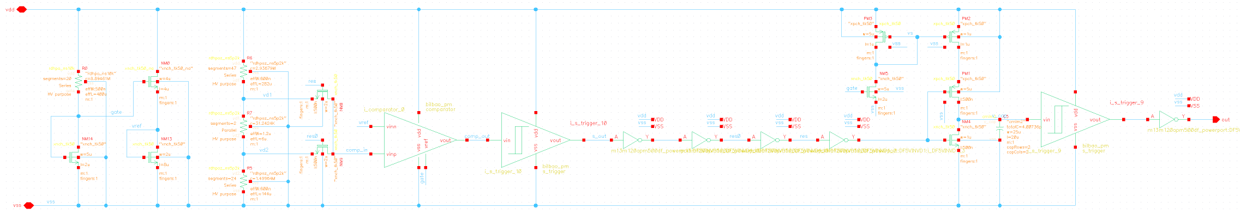
\includegraphics[keepaspectratio, scale=0.7, angle=-90]{figures/CD/Picture1.png}};

        % Berechnung der Mittelpunkte für die Beschriftung
        \pgfmathsetmacro{\ymidA}{(0 + 7)/2}
        \pgfmathsetmacro{\ymidB}{(7 + 13.5)/2}    % Mittelpunkt für "Schaltpunkte Komparator"
        \pgfmathsetmacro{\ymidC}{(13.5 + 18.5)/2} % Mittelpunkt für "Inverterkette"
        \pgfmathsetmacro{\ymidD}{(18.5 + 23)/2}   % Mittelpunkt für "Generierung Referenzstrom"

        \begin{scope}
            % Gestrichelte Linien
            \draw[dashed] (0,7) -- ++(10,0);
            \draw[dashed] (0,13.5) -- ++(10,0);
            \draw[dashed] (0,18.5) -- ++(10,0);

            % Mittelpunkte setzen (berechnete Werte werden nun genutzt)
            \node at (8, \ymidA) {\textbf{Verzögerungs- und Reset-Element}};
            \node at (8, \ymidB) {\textbf{Inverterkette}};
            \node at (8, \ymidC) {\textbf{Schaltpunkte Komparator}};
            \node at (8, \ymidD) {\textbf{Generierung Referenzstrom}};
        \end{scope}
    \end{tikzpicture}
    \caption{Schaltbild der kompletten PoR-Schaltung}
    \label{fig:PoR_complete}
\end{figure}


\begin{figure}[H]
    \centering
    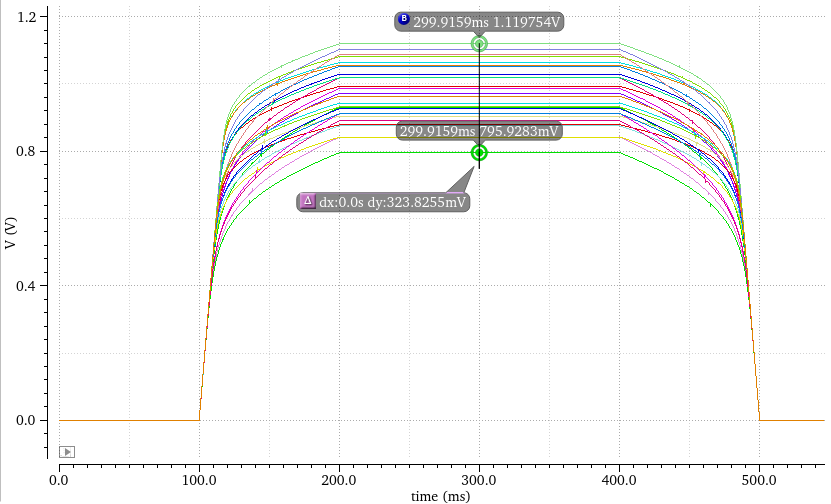
\includegraphics[width=\linewidth]{figures/CD/vref_old.png}
    \caption{Schwankung der Referenzspannung mit Widerstand}
    \label{fig:Vref_fluctuation_old}
    \addcontentsline{app}{figure}{\protect\numberline{\thefigure} Schwankung der Referenzspannung mit Widerstand}
\end{figure}

\begin{figure}[H]
    \centering
    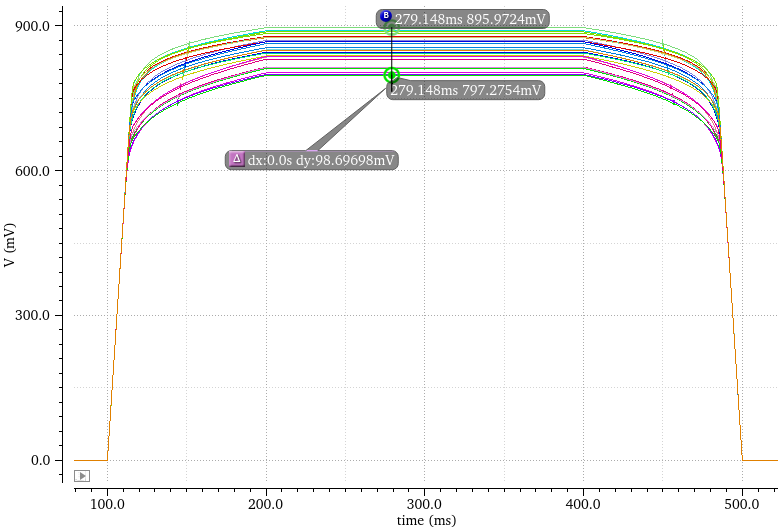
\includegraphics[width=\linewidth]{figures/CD/vref_test1.png}
    \caption{Schwankung der Referenzspannung mit Transistoren}
    \label{fig:Vref_Variation}
    \addcontentsline{app}{figure}{\protect\numberline{\thefigure} Schwankung der Referenzspannung mit Transistoren}
\end{figure}

\chapter{Tabellen}\label{apdx:B}

% Nummerierung auf A1, A2, etc. umstellen
\renewcommand{\thetable}{B.\arabic{table}}
\setcounter{table}{0} % Zähler zurücksetzen

%\section{Tabellen}\label{sec:apdx:Tabellen}

\begin{table}[H]
    \centering
    \small
    \begin{tabular}{c|l|c|c|c}
        {\rotatebox{90}{\parbox{1.8cm}{\textbf{Spannung}}}} &
        \textbf{\makecell{Werte}} &
        \textbf{\makecell{Spezifikation}} &
        \textbf{\makecell{Min. Wert}} &
        \textbf{\makecell{Max. Wert}} \\
        \midrule

        \multirow{5}{*}{\rotatebox{90}{5 V}} &
        Verzögerung steigende Flanke & 20 us $\leq$ x $\leq$ 130 us & 46.14 us & 89.68 us \\
        & Verzögerung fallende Flanke & x $\leq$ 1 us & 57.79 ns & 80.07 ns \\
        & Schwellspannung steigend & 2.2 V $\leq$ x $\leq$ 2.6 V & \cellcolor{lightred}2.093 V & \cellcolor{lightred}2.726 V \\
        & Schwellspannung fallend & 2.1 V $\leq$ x $\leq$ 2.5 V & \cellcolor{lightred}2.033 V & \cellcolor{lightred}2.655 V \\
        & Hysterese & 50 mV $\leq$ x $\leq$ 120 mV & 59.2 mV & 71.26 mV \\
        \midrule

        \multirow{5}{*}{\rotatebox{90}{1.5 V}} &
        Verzögerung steigende Flanke & 20 us $\leq$ x $\leq$ 230 us & 42.39 us & 77.62 us \\
        & Verzögerung fallende Flanke & x $\leq$ 1 us & 80.16 ns & 118.7 ns \\
        & Schwellspannung steigend & 1.1 V $\leq$ x $\leq$ 1.45 V & 1.148 V & 1.1445 V \\
        & Schwellspannung fallend & 1.05 V $\leq$ x $\leq$ 1.4 V & 1.079 V & 1.36 V \\
        & Hysterese & 50 mV $\leq$ x $\leq$ 120 mV & 68.96 mV & 84.8 mV \\
        \midrule
        
    \end{tabular}
    \caption{MC-Process-Simulation mit Anstiegs-und Abfallzeit von 10~ms}
    \label{tab:MCProcess10}
\end{table}
\addcontentsline{app}{table}{\protect\numberline{\thetable} Monte-Carlo-Ergebnisse für 10 ms Process}

\begin{table}[H]
    \centering
    \small
    \begin{tabular}{c|l|c|c|c}
        {\rotatebox{90}{\parbox{1.8cm}{\textbf{Spannung}}}} &
        \textbf{\makecell{Werte}} &
        \textbf{\makecell{Spezifikation}} &
        \textbf{\makecell{Min. Wert}} &
        \textbf{\makecell{Max. Wert}} \\
        \midrule
        
        \multirow{5}{*}{\rotatebox{90}{5 V}} &
        Verzögerung steigende Flanke & 20 us $\leq$ x $\leq$ 130 us & 40.14 us & 109.5 us \\
        & Verzögerung fallende Flanke & x $\leq$ 1 us & 64.04 ns & 72.13 ns \\
        & Schwellspannung steigend & 2.2 V $\leq$ x $\leq$ 2.6 V & 2.354 V & 2.461 V \\
        & Schwellspannung fallend & 2.1 V $\leq$ x $\leq$ 2.5 V & 2.289 V & 2.396 V \\
        & Hysterese & 50 mV $\leq$ x $\leq$ 120 mV & 62.34 mV & 66.29 mV \\
        \midrule

        \multirow{5}{*}{\rotatebox{90}{1.5 V}} &
        Verzögerung steigende Flanke & 20 us $\leq$ x $\leq$ 230 us & 33.84 us & 77.87 us \\
        & Verzögerung fallende Flanke & x $\leq$ 1 us & 84.91 ns & 108 ns \\
        & Schwellspannung steigend & 1.1 V $\leq$ x $\leq$ 1.45 V & 1.22 V & 1.344 V \\
        & Schwellspannung fallend & 1.05 V $\leq$ x $\leq$ 1.4 V & 1.146 V & 1.264 V \\
        & Hysterese & 50 mV $\leq$ x $\leq$ 120 mV & 73.58 mV & 79.58 mV \\
        \midrule
        
    \end{tabular}
    \caption{MC-Mismatch-Simulation mit Anstiegs-und Abfallzeit von 10~ms}
    \label{tab:MCMismatch10}
\end{table}
\addcontentsline{app}{table}{\protect\numberline{\thetable} Monte-Carlo-Ergebnisse für 10 ms Mismatch}

\begin{table}[H]
    \centering
    \small
    \begin{tabular}{c|l|c|c|c}
        {\rotatebox{90}{\parbox{1.8cm}{\textbf{Spannung}}}} &
        \textbf{\makecell{Werte}} &
        \textbf{\makecell{Spezifikation}} &
        \textbf{\makecell{Min. Wert}} &
        \textbf{\makecell{Max. Wert}} \\
        \midrule

        \multirow{5}{*}{\rotatebox{90}{5 V}} &
        Verzögerung steigende Flanke & 20 us $\leq$ x $\leq$ 130 us & 39.05 us & 116.2 us \\
        & Verzögerung fallende Flanke & x $\leq$ 1 us & 57.3 ns & 81.9 ns \\
        & Schwellspannung steigend & 2.2 V $\leq$ x $\leq$ 2.6 V & \cellcolor{lightred}2.063 V & \cellcolor{lightred}2.755 V \\
        & Schwellspannung fallend & 2.1 V $\leq$ x $\leq$ 2.5 V & \cellcolor{lightred}2.003 V & \cellcolor{lightred}2.682 V \\
        & Hysterese & 50 mV $\leq$ x $\leq$ 120 mV & 58.8 mV & 72.8 mV \\
        \midrule

        \multirow{5}{*}{\rotatebox{90}{1.5 V}} &
        Verzögerung steigende Flanke & 20 us $\leq$ x $\leq$ 230 us & 36.95 us & 88.95 us \\
        & Verzögerung fallende Flanke & x $\leq$ 1 us & 77.28 ns & 129.3 ns \\
        & Schwellspannung steigend & 1.1 V $\leq$ x $\leq$ 1.45 V & 1.123 V & \cellcolor{lightyellow}1.452 V \\
        & Schwellspannung fallend & 1.05 V $\leq$ x $\leq$ 1.4 V & 1.055 V & 1.368 V \\
        & Hysterese & 50 mV $\leq$ x $\leq$ 120 mV & 68.02 mV & 84.34 mV \\
        \midrule
        
    \end{tabular}
    \caption{MC-All-Simulation mit Anstiegs-und Abfallzeit von 10~ms}
    \label{tab:MCAll10}
\end{table}
\addcontentsline{app}{table}{\protect\numberline{\thetable} Monte-Carlo-Ergebnisse für 10 ms All}

\begin{table}[H]
    \centering
    \small
    \begin{tabular}{c|l|c|c|c}
        {\rotatebox{90}{\parbox{1.8cm}{\textbf{Spannung}}}} &
        \textbf{\makecell{Werte}} &
        \textbf{\makecell{Spezifikation}} &
        \textbf{\makecell{Min. Wert}} &
        \textbf{\makecell{Max. Wert}} \\
        \midrule

        \multirow{5}{*}{\rotatebox{90}{5 V}} &
        Verzögerung steigende Flanke & 20 ms $\leq$ x $\leq$ 130 ms & 40.16 ms & 122.4 ms \\
        & Verzögerung fallende Flanke & x $\leq$ 1 ms & 57.8 ns & 82.86 ns \\
        & Schwellspannung steigend & 2.2 V $\leq$ x $\leq$ 2.6 V & \cellcolor{lightred}2.081 V & \cellcolor{lightred}2.77 V \\
        & Schwellspannung fallend & 2.1 V $\leq$ x $\leq$ 2.5 V & \cellcolor{lightred}1.985 V & \cellcolor{lightred}2.667 V \\
        & Hysterese & 50 mV $\leq$ x $\leq$ 120 mV & 84.68 mV & 104.4 mV \\
        \midrule

        \multirow{5}{*}{\rotatebox{90}{1.5 V}} &
        Verzögerung steigende Flanke & 20 ms $\leq$ x $\leq$ 230 ms & 37.02 ms & 89 ms \\
        & Verzögerung fallende Flanke & x $\leq$ 1 ms & 77.56 ns & 129.9 ns \\
        & Schwellspannung steigend & 1.1 V $\leq$ x $\leq$ 1.45 V & 1.126 V & \cellcolor{lightyellow}1.454 V \\
        & Schwellspannung fallend & 1.05 V $\leq$ x $\leq$ 1.4 V & 1.052 V & 1.366 V \\
        & Hysterese & 50 mV $\leq$ x $\leq$ 120 mV & 72.96 mV & 87.6 mV \\
        \midrule
        
    \end{tabular}
    \caption{MC-All-Simulation mit Anstiegs-und Abfallzeit von 1~ms}
    \label{tab:MCAll1}
\end{table}
\addcontentsline{app}{table}{\protect\numberline{\thetable} Monte-Carlo-Ergebnisse für 1 ms All}
%
% Ende
%
\pagestyle{plain}
\include{frontbackmatter/Acknowledgements}
\ifthenelse{\boolean{frontdeclaration}}{}{%
    \begingroup
\cleardoublepage

%
% Bei Verwendung von Part (Teil) nicht entfernen!
% Dies sorgt dafür, dass die PDF-Lesezeichen in der
% richtigen Hierarchieebene liegen.
\pdfbookmark[-1]{Erklärung an Eides statt}{pdf-Declaration}
%
\chapter*{Erklärung an Eides statt}
\addcontentsline{toc}{chapter}{Erklärung an Eides statt}
Ich erkläre an Eides statt, dass ich die vorliegende Arbeit selbständig und ohne unerlaubte fremde Hilfe angefertigt, andere als die angegebenen Quellen und Hilfsmittel nicht benutzt habe. Die aus fremden Quellen direkt oder indirekt übernommenen Stellen sind als solche kenntlich gemacht.
\medskip

\noindent Die Zustimmung des Partnerunternehmens in der Praxis zur Verwendung betrieblicher Unterlagen habe ich eingeholt. Die Arbeit wurde bisher in gleicher oder ähnlicher Form keiner anderen Prüfungsbehörde vorgelegt und auch nicht veröffentlicht
\bigskip

\noindent\textit{\myLocation, \myDeclarationDate}

\smallskip

\begin{flushright}
    \begin{tabular}{m{5cm}}
        \\ \hline
        \centering\myName \\
    \end{tabular}
\end{flushright}
\endgroup%
}
\end{document}